\documentclass[10pt, a4paper]{article}

% Parametri che modificano il file main.tex
% Le uniche parti da cambiare su main.tex sono:
% - vari \vspace tra sezioni
% - tabella azioni da intraprendere
% - sezione altro

\def\data{2024-03-12}
\def\oraInizio{14:00}
\def\oraFine{15:30}
\def\luogo{Piattaforma Discord}

\def\tipoVerb{Interno} % Interno - Esterno

\def\nomeResp{Orlandi G.} % Cognome N.
\def\nomeVer{Bresolin G.} % Cognome N.
\def\nomeSegr{Michelon R.} % Cognome N.

\def\nomeAzienda{Azzurro Digitale}
\def\firmaAzienda{azzurrodigitale.png}
\def\firmaResp{giacomo.png} % nome Responsabile

\def\listaPartInt{
Bresolin G.,
Campese M.,
Ciriolo I.,
Dugo A.,
Feltrin E.,
Michelon R.,
Orlandi G.
}

\def\listaPartEst{
Azzurro B.,
Digitale C.,
}

% Se nessuna revisione: \def\listaRevisioneAzioni {x}
\def\listaRevisioneAzioni {x}

\def\listaOrdineGiorno {
{Aggiornamento da parte di tutti i membri del gruppo riguardo al lavoro di codifica iniziato dopo la riunione precedente;},
{Preparazione per la riunione con l'azienda pianificata in data 2024-03-13;},
{Assegnazione dei task relativi alla parte di testing.}
}

\def\listaDiscussioneInterna {
{Il team ha eseguito un aggiornamento generale relativo alla codifica del backend in corso da una settimana. Considerati i buoni risultati il gruppo ha discusso della possibilità di presentare il lavoro svolto durante la riunione con AzzurroDigitale pianificata per il 2024-03-13;},
{Il team ha riportato la discussione tenuta in settimana per la divisione del lavoro da svolgere riguardante la parte di test di unità delle componenti sviluppate durante la prima parte di codifica del progetto. La suddivisione delle task viene quindi riportata in 'Azioni da intraprendere'.
}
}



% Se nessuna decisione: \def\listaDecisioni {x}
\def\listaDecisioni{
{Il team presenterà all'azienda il lavoro di codifica delle componenti di backend svolto fino ad ora;},
{Il team continuerà la produzione della parte di test di unità delle componenti di backend secondo la suddivisione dei compiti riportata in 'Azioni da intraprendere'.}
}

\setcounter{secnumdepth}{5}
\setcounter{tocdepth}{5}
\makeatletter
\newcommand\subsubsubsection{\@startsection{paragraph}{4}{\z@}{-2.5ex\@plus -1ex \@minus -.25ex}{1.25ex \@plus .25ex}{\normalfont\normalsize\bfseries}}
\newcommand\subsubsubsubsection{\@startsection{subparagraph}{5}{\z@}{-2.5ex\@plus -1ex \@minus -.25ex}{1.25ex \@plus .25ex}{\normalfont\normalsize\bfseries}}
\makeatother

\usepackage{style}
\usepackage{headerfooter}
\usepackage{comment}

\title{\titolo}
\author{SWEetCode}

\begin{document}

% PRIMA PAGINA
\begin{titlepage}
    \thispagestyle{empty}
    \begin{tikzpicture}[remember picture, overlay]
        % TRIANGOLI
        \draw[fill=secondarycolor, secondarycolor] (current page.north west) -- (current page.south west) -- (8.8, -28);
        \draw[fill=primarycolor, primarycolor] (-3, 5) -- (4, -13.6) -- (11, 5);

        % LOGO
        \node [xshift=-5cm, yshift=25cm] (logo) at (current page.south east) {
\includegraphics[width=6.5cm]{img/logo.png}};

        % SWEETCODE - DATE
        \node [anchor=north east, align=right, xshift=-1.2cm, yshift=20.5cm, text=black] (sweetcode) at (current page.south east) {\fontsize{32pt}{36pt}\selectfont SWEetCode};
        \draw[line width=4pt, lightcol] ([xshift=-3cm, yshift=-0.37cm]sweetcode.south west) -- ([yshift=-0.37cm]sweetcode.south east);
        \node [anchor=north east, align=right, xshift=-1.2cm, yshift=18.7cm, text=black] (date) at (current page.south east){\fontsize{24pt}{24pt} \selectfont Verbale \tipoVerb};

        % NOME FILE
        \node [anchor=north east, text width=15cm, align=right, xshift=-1.2cm, yshift=17cm, text=black] (titolo) at (current page.south east){\fontsize{48pt}{48pt}\textbf{\data}};

        % BOX DATI PARTECIPANTI
        \ifthenelse{\equal{\tipoVerb}{Esterno}}{
            \node[anchor=north east, xshift=-1.2cm, yshift=14.5cm, minimum width=8cm] (box) at (current page.south east){};
        }{
            \node[anchor=north east, xshift=-1.2cm, yshift=12.5cm, minimum width=8cm] (box) at (current page.south east){};
        }

        % RESPONSABILE
        \node[anchor=north west, align=left] (dati2) at (box.north west) {\fontsize{15pt}{15pt}\selectfont \textbf{Responsabile}};
        \draw[line width=4pt, lightcol] (dati2.south west) -- ([xshift=8cm]dati2.south west);
        \node[anchor=north west, align=left] (dati21) at (dati2.south west){\fontsize{13pt}{13pt}\selectfont \nomeResp};

        % VERIFICATORE
        \node[anchor=north west, yshift=-1cm, align=left] (dati3) at (dati21.north west) {\fontsize{15pt}{15pt}\selectfont \textbf{Verificatore}};
        \draw[line width=4pt, lightcol] (dati3.south west) -- ([xshift=8cm]dati3.south west);
        \node[anchor=north west, align=left] (dati31) at (dati3.south west){\fontsize{13pt}{13pt}\selectfont \nomeVer};

        % SEGRETARIO DI RIUNIONE
        \node[anchor=north west, yshift=-1cm, align=left] (dati4) at (dati31.north west) {\fontsize{15pt}{15pt}\selectfont \textbf{Segretario di Riunione}};
        \draw[line width=4pt, lightcol] (dati4.south west) -- ([xshift=8cm]dati4.south west);
        \node[anchor=north west, align=left] (dati41) at (dati4.south west){\fontsize{13pt}{13pt}\selectfont \nomeSegr};
        
        % UNIPD - SWE
        \node [xshift=4.4cm, yshift=2.3cm, draw, secondarycolor, text=white] (uni) at (current page.south west) {\fontsize{20pt}{20pt} \selectfont Università di Padova};
        \node [xshift=0.65cm, yshift=0.7cm, draw, secondarycolor, text=white, below=of uni] (corso) {\fontsize{20pt}{20pt}\selectfont Ingegneria del Software};

        % FIRMA AZIENDA
        %\ifthenelse{\equal{\tipoVerb}{Esterno}}{
           % \draw[line width=4pt, lightcol] ([xshift=-1.2cm, yshift=5.2cm]current page.south east) -- ([xshift=-8cm, yshift=5.2cm]current page.south east);
          %  \node [xshift=-4.8cm, yshift=6.3cm] (logo) at (current page.south east) {\includegraphics[width=6cm]{img/firme/\firmaAzienda}};
          %  \node[anchor=north west, xshift=12.9cm, yshift=4.95cm, align=left] at (current page.south west)
           % {\fontsize{13pt}{13pt}\selectfont L'azienda: \nomeAzienda};
       % }

       %  FIRMA
        \draw[line width=4pt, lightcol] ([xshift=-1.2cm, yshift=1.8cm]current page.south east) -- ([xshift=-8cm, yshift=1.8cm]current page.south east);
        \node [xshift=-4.8cm, yshift=2.45cm] (logo) at (current page.south east) {\includegraphics[width=6cm]{img/firme/\firmaResp}};
        \node[anchor=north west, xshift=12.9cm, yshift=1.45cm, align=left] at (current page.south west)
        {\fontsize{13pt}{13pt}\selectfont Il Responsabile: \nomeResp};
        
    \end{tikzpicture}
\end{titlepage}

% REGISTRO DELLE VERSIONI
%Registro in ordine dalla più recente alla meno recente!

{\renewcommand{\arraystretch}{1.5}
\section*{Registro delle versioni}

\begin{xltabular}{\textwidth}{c|c|c|c|X}
\label{tab:long}

\textbf{Versione} & \textbf{Data} & \quantities{\textbf{Responsabile di}\\\textbf{stesura}}& \textbf{Revisore} & \quantities{\textbf{Dettaglio e}\\\textbf{motivazioni}} \\
\endfirsthead

\textbf{Versione} & \textbf{Data} & \quantities{\textbf{Responsabile di}\\\textbf{stesura}}& \textbf{Revisore} & \quantities{\textbf{Dettaglio e}\\\textbf{motivazioni}} \\
\endhead

\multicolumn{5}{r}{{Continua nella pagina successiva}} \\
\endfoot

\endlastfoot

\hline
v2.23.0(1) & $2024-03-20$ & \quantities{Ciriolo I.} & Feltrin E. & Gestione e visualizzazione delle chat.\\
\hline
v2.21.0(1) & $2024-03-19$ & \quantities{Ciriolo I.} & Michelon R. & Prima stesura.\\
\hline
    
\end{xltabular}}
\newpage

% INDICE
\tableofcontents
\newpage
\listoffigures
\newpage
\listoftables
\newpage

% INTRODUZIONE
\section{Introduzione}
\subsection{Obiettivo del documento}
L'obiettivo che ci si pone nella realizzazione di questo documento è la definizione delle metriche di valutazione e validazione del progetto, e la specifica degli obiettivi di qualità del prodotto finale. Tali parametri vengono stabiliti in accordo ai requisiti e 
alle aspettative del proponente e talvolta a discrezione del team sulla base delle valutazioni fatte nel corso di studi.

\subsection{Glossario}
Per evitare ambiguità ed incomprensioni relative al linguaggio e ai termini utilizzati nella documentazione del progetto viene presentato un Glossario.
I termini ambigui o tecnici-specifici presenti nello stesso, vengono identificati nei corrispondenti documenti con un pedice |g| e con una scrittura in corsivo.
All'interno dei documenti viene identificata con tale scrittura solo e soltanto la prima occorrenza presente nel testo di un termine definito nel Glossario.

\subsection{Riferimenti}
   \subsubsection{Riferimenti normativi}
   \begin{itemize}
    \item \textit{Guidelines for the application of ISO/IEC 90003:2004 to computer software}: \\
        \url{https://cdn.standards.iteh.ai/samples/35867/36860aa4caba4c84b26051db576456d3/ISO-IEC-90003-2004.pdf}\\
        (Ultimo accesso: 2024-02-08);
    \item \textit{(Norme di progetto v2.0.0(0))};
    \item \textit{Regolamento del progetto didattico}: \\
        \url{https://www.math.unipd.it/~tullio/IS-1/2023/Dispense/PD2.pdf}\\
        (Ultimo accesso: 2024-02-08);
    \item \textit{Standard ISO/IEC 9126}:\\
        \url{https://it.wikipedia.org/wiki/ISO/IEC_9126}\\
        (Ultimo accesso: 2024-02-08).
    \end{itemize}
    
    \subsubsection{Riferimenti informativi}
    \begin{itemize}
        \item \textit{(Analisi dei requisiti v2.0.0(0))};
        \item \textit{Capitolato C1}: \textit{Knowledge Management AI}
        \begin{itemize}
            \item \url{https://www.math.unipd.it/~tullio/IS-1/2023/Progetto/C1.pdf}\\
            (Ultimo accesso: 2024-02-08);
            \item \url{https://www.math.unipd.it/~tullio/IS-1/2023/Progetto/C1p.pdf}\\
            (Ultimo accesso: 2024-02-08).
        \end{itemize}
        \item \textit{Dispense sulla Qualità di processo (argomento T8)}: \\
            \url{https://www.math.unipd.it/~tullio/IS-1/2023/Dispense/T8.pdf}\\
            (Ultimo accesso: 2024-02-08);
        \item \textit{Dispense sulla Verifica e Validazione: Introduzione (argomento T9)}: \\
            \url{https://www.math.unipd.it/~tullio/IS-1/2023/Dispense/T9.pdf}\\
            (Ultimo accesso: 2024-02-08).
        \item \textit{(Glossario v2.0.0(0))};
        \item \textit{(Piano di progetto v2.0.0(0))};
        \item \textit{Verbali esterni ed interni}.
    \end{itemize}

    
% Obiettivi di qualità
\newpage
\section{Obiettivi di qualità}
\label{ObiettiviQualità}
Per garantire la qualità di processo si è deciso di aderire agli standard ISO/IEC 90003:2004 e ISO/IEC 9126 e agli obiettivi di qualità da essi previsti. In questa sezione si presentano i valori accettabili e ideali delle metriche sulle quali si basano questi obiettivi; le definizioni di tali metriche sono riportate in (Norme di progetto v2.0.0, \S Lista delle metriche).
\subsection{Qualità di processo}
%\paragraph{}breve descrizione qualità di processo da inserire.\\
\renewcommand{\arraystretch}{1.5}
%\begin{table}[H]
\begin{xltabular}{\textwidth}{p{0.13\textwidth}|p{0.5\textwidth}|X|X}


\textbf{ID} & \textbf{Nome metrica} & \textbf{Valore tollerabile} & \textbf{Valore ambito}   \\
\endfirsthead

\textbf{ID} & \textbf{Nome metrica} & \textbf{Valore tollerabile} & \textbf{Valore ambito}   \\
\endhead
\caption{Metriche per la qualità di processo (cont.)}\\
\multicolumn{4}{r}{\footnotesize\textit{Continua nella pagina successiva}} \\
\endfoot
\caption[]{Metriche per la qualità di processo}\\

\endlastfoot

\hline
M.PC.1.PMS & Percentuale di metriche soddisfatte & $ \ge75\% $& $ 100\% $\\
\hline
M.PC.2.RNP & Rischi non previsti & $ \le2 $ & $ 0 $\\
\hline
M.PC.3.VP & Variazione di piano & $ \le1 $ & $ 0 $ \\
\hline
M.PC.4.VC & Variazione di costo & $ 0 $ & $ \ge100 $ \\
\hline
M.PC.5.ISR &  Indice di stabilità dei requisiti & $ \ge70\% $ & $ 100\% $  \\
\hline
M.PC.6.CCM & Complessità ciclomatica media & $\le6 $ & $\le3 $ \\
\hline
M.PC.7.SC & Statement coverage & $ \ge90\% $ & $ 100\% $ \\
\hline
M.PC.8.BC & Branch coverage & $ \ge90\% $ & $ 100\% $ \\
\hline
M.PC.9.ET & Efficienza temporale & $ \le140\% $ & $ 100\% $ \\
\end{xltabular}
    
\subsection{Qualità di prodotto}
Abbiamo analizzato quali caratteristiche fossero necessarie per la realizzazione di un prodotto di 
qualità.\\

\renewcommand{\arraystretch}{1.5}
%\begin{table}[H]
\begin{xltabular}{\textwidth}{p{0.13\textwidth}|p{0.5\textwidth}|X|X}


\textbf{ID} & \textbf{Nome metrica} & \textbf{Valore tollerabile} & \textbf{Valore ambito}   \\
\endfirsthead

\textbf{ID} & \textbf{Nome metrica} & \textbf{Valore tollerabile} & \textbf{Valore ambito}   \\
\endhead
\caption{Metriche per la qualità di prodotto (cont.)}\\
\multicolumn{4}{r}{\footnotesize\textit{Continua nella pagina successiva}} \\
\endfoot
\caption[]{Metriche per la qualità di prodotto}\\

\endlastfoot


\hline
M.PD.1.IG & Indice di Gulpease & $ \ge60\% $& $\ge80\% $\\
\hline
M.PD.2.LMC & Linee medie di codice per metodo & $\le30$ & $\le20$ \\
\hline
M.PD.3.AFS &  Adeguatezza delle funzioni sviluppate &-& - \\
\hline
M.PD.4.AR &  Accuratezza della risposta &-& - \\
\hline
M.PD.5.RD &  Rimozione dei difetti &-& - \\
\hline
M.PD.6.LCG &   Livello di controllo dei guasti &-& - \\

\hline
M.PD.7.CD &  Completezza descrittiva &-& - \\
\hline
M.PD.8.IM & Impatto delle modifiche &-& - \\

\hline
M.PD.9.TS & Percentuale di test superati  & $ \ge90\% $& $100\%$\\
    \hline
M.PD.10.CSD & Correttezza dello scambio di dati (Percezione degli utenti) &-& - \\
\hline
M.PD.11.AFPH &Accesso fisico alle funzioni da  parte di personale portatore di handicap &-& - \\
\hline
M.PD.12.TR & Tempo di risposta &-& - \\
\hline
M.PD.13.EI & Efficienza dell’installazione &-& - \\
   
 

\end{xltabular}
%\caption{Metriche per la qualità di prodotto}
%\end{table}}

    
%\subsection{Software}





\subsection{Qualità per obiettivo}
\subsubsection{Processi primari}
 
\subsubsubsection{Fornitura}

\renewcommand{\arraystretch}{1.5}
\begin{table}[H]
\begin{xltabular}{\textwidth}{p{0.13\textwidth}|p{0.5\textwidth}|X|X}


\textbf{ID} & \textbf{Nome metrica} & \textbf{Valore tollerabile} & \textbf{Valore ambito}   \\
\endfirsthead

\textbf{ID} & \textbf{Nome metrica} & \textbf{Valore tollerabile} & \textbf{Valore ambito}   \\
\endhead

\multicolumn{4}{r}{{Continua nella pagina successiva}} \\
\endfoot

\endlastfoot

\hline
M.PC.3.VP & Variazione di piano & $ \le1 $ & $ 0 $ \\
\hline
M.PC.4.VC & Variazione di costo & $ 0 $ & $ \ge100 $ \\

\end{xltabular}
\caption{Metriche per la fornitura}
\end{table}


 
\subsubsubsection{Sviluppo}

\subsubsubsubsection{Analisi dei requisiti}
\renewcommand{\arraystretch}{1.5}
\begin{table}[H]
\begin{xltabular}{\textwidth}{p{0.13\textwidth}|p{0.5\textwidth}|X|X}

\textbf{ID} & \textbf{Nome metrica} & \textbf{Valore tollerabile} & \textbf{Valore ambito}   \\
\endfirsthead

\textbf{ID} & \textbf{Nome metrica} & \textbf{Valore tollerabile} & \textbf{Valore ambito}   \\
\endhead

\multicolumn{4}{r}{{Continua nella pagina successiva}} \\
\endfoot

\endlastfoot
\hline
M.PC.5.ISR &  Indice di stabilità dei requisiti & $ \ge70\% $ & $ 100\% $  \\
\end{xltabular}
\caption{Metriche per l'analisi dei requisiti}
\end{table}

\subsubsubsubsection{Codifica}
\renewcommand{\arraystretch}{1.5}
\begin{table}[H]
\begin{xltabular}{\textwidth}{p{0.13\textwidth}|p{0.5\textwidth}|X|X}

\textbf{ID} & \textbf{Nome metrica} & \textbf{Valore tollerabile} & \textbf{Valore ambito}   \\
\endfirsthead

\textbf{ID} & \textbf{Nome metrica} & \textbf{Valore tollerabile} & \textbf{Valore ambito}   \\
\endhead

\multicolumn{4}{r}{{Continua nella pagina successiva}} \\
\endfoot

\endlastfoot
\hline
M.PC.6.CCM & Complessità ciclomatica media & $\le6 $ & $\le3 $ \\
\hline
M.PC.7.SC & Statement coverage & $ \ge90\% $ & $ 100\% $ \\
\hline
M.PC.8.BC & Branch Coverage & $ \ge90\% $ & $ 100\% $ \\
\hline
M.PD.2.LMC & Linee medie di codice per metodo & $\le30$ & $\le20$ \\
       

\end{xltabular}
\caption{Metriche per la codifica}
\end{table}

\subsubsubsubsection{Testing}
\renewcommand{\arraystretch}{1.5}
\begin{table}[H]
\begin{xltabular}{\textwidth}{p{0.13\textwidth}|p{0.5\textwidth}|X|X}

\textbf{ID} & \textbf{Nome metrica} & \textbf{Valore tollerabile} & \textbf{Valore ambito}   \\
\endfirsthead

\textbf{ID} & \textbf{Nome metrica} & \textbf{Valore tollerabile} & \textbf{Valore ambito}   \\
\endhead

\multicolumn{4}{r}{{Continua nella pagina successiva}} \\
\endfoot

\endlastfoot

\hline
M.PD.9.TS & Percentuale di test superati  & $ \ge90\% $& $100\%$\\
\hline
M.PD.3.AFS &  Adeguatezza delle funzioni sviluppate &-& - \\
\hline
M.PD.8.IM & Impatto delle modifiche &-& - \\
\hline
M.PD.10.CSD & Correttezza dello scambio di dati (Percezione degli utenti) &-& - \\

    
\end{xltabular}
\caption{Metriche per il testing}
\end{table}
 
   
% PROCESSI DI SUPPORTO
\subsubsection{Processi di supporto}
\subsubsubsection{Documentazione}
\renewcommand{\arraystretch}{1.5}
\begin{table}[H]
\begin{xltabular}{\textwidth}{p{0.13\textwidth}|p{0.5\textwidth}|X|X}

\textbf{ID} & \textbf{Nome metrica} & \textbf{Valore tollerabile} & \textbf{Valore ambito}   \\
\endfirsthead

\textbf{ID} & \textbf{Nome metrica} & \textbf{Valore tollerabile} & \textbf{Valore ambito}   \\
\endhead

\multicolumn{4}{r}{{Continua nella pagina successiva}} \\
\endfoot

\endlastfoot
\hline
M.PD.1.IG & Indice di Gulpease & $ \ge60\% $& $\ge80\% $\\
\hline
M.PD.7.CD &  Completezza descrittiva &-& - \\
\end{xltabular}
\caption{Metriche per la documentazione}
\end{table}

\begin{comment}
%\subsubsection{Documentazione}
    \renewcommand{\arraystretch}{1.5}
    \begin{tabularx}{\textwidth}{p{0.18\textwidth}|p{0.6\textwidth}|X}
    \textbf{Obiettivo} & \textbf{Descrizione} & \textbf{Metriche}  \\
    \hline
    Correttezza Risposte &   & \\
    \hline
    Velocità di esecuzione &  &  \\
    \end{tabularx}
    \renewcommand{\arraystretch}{1.5}
    \begin{tabularx}{\textwidth}{p{0.18\textwidth}|p{0.6\textwidth}|X}
    \textbf{Obiettivo} & \textbf{Descrizione} & \textbf{Metriche}  \\
    \hline
    Verifica &  &  \\
    \hline
    Gestione della qualità &  &  \\
    \end{tabularx}
\end{comment}    

\subsubsubsection{Assicurazione della qualità}
\renewcommand{\arraystretch}{1.5}
\begin{table}[H]
\begin{xltabular}{\textwidth}{p{0.13\textwidth}|p{0.5\textwidth}|X|X}

\textbf{ID} & \textbf{Nome metrica} & \textbf{Valore tollerabile} & \textbf{Valore ambito}   \\
\endfirsthead

\textbf{ID} & \textbf{Nome metrica} & \textbf{Valore tollerabile} & \textbf{Valore ambito}   \\
\endhead

\multicolumn{4}{r}{{Continua nella pagina successiva}} \\
\endfoot

\endlastfoot
\hline
    M.PD.4.AR &  Accuratezza della risposta &-& - \\
        
    \hline
    M.PD.5.RD &  Rimozione dei difetti &-& - \\
   \hline
    M.PD.6.LCG &   Livello di controllo dei guasti &-& - \\
    \hline
   M.PD.11.AFPH &Accesso fisico alle funzioni da  parte di personale portatore di handicap &-& - \\
    \hline
 M.PD.12.TR & Tempo di risposta &-& - \\
   \hline
M.PD.13.EI & Efficienza dell’installazione &-& - \\

\end{xltabular}
\caption{Metriche per la assicurazione della qualità}
\end{table}

 % PROCESSI ORGANIZZATIVI   
\subsubsection{Processi organizzativi}
\renewcommand{\arraystretch}{1.5}
\begin{table}[H]
\begin{xltabular}{\textwidth}{p{0.13\textwidth}|p{0.5\textwidth}|X|X}

\textbf{ID} & \textbf{Nome metrica} & \textbf{Valore tollerabile} & \textbf{Valore ambito}   \\
\endfirsthead

\textbf{ID} & \textbf{Nome metrica} & \textbf{Valore tollerabile} & \textbf{Valore ambito}   \\
\endhead

\multicolumn{4}{r}{{Continua nella pagina successiva}} \\
\endfoot

\endlastfoot
\hline
M.PC.2.RNP & Rischi non previsti & $ \le2 $ & $ 0 $\\
\end{xltabular}
\caption{Metriche per i processi organizzativi}
\end{table}
\begin{comment}
    \renewcommand{\arraystretch}{1.5}
    \begin{tabularx}{\textwidth}{p{0.18\textwidth}|p{0.6\textwidth}|X}
    \textbf{Obiettivo} & \textbf{Descrizione} & \textbf{Metriche}  \\
    \hline
    Gestione organizzativa &  &  \\
    \end{tabularx}
\end{comment}

%Test e specifiche
\newpage
\section{Verifica}

\subsection{Test di unità}
Di seguito vengono elencati i test di unità:


\renewcommand{\arraystretch}{1.5}
\begin{xltabular}{\textwidth}{p{0.12\textwidth}|p{0.7\textwidth}|X}
\textbf{ID} & \textbf{Descrizione} & \textbf{Stato}  \\
\hline
TU1 & Verifica che il metodo toDocument di NewDocument gestisca correttamente un documento PDF & S \\
\hline
TU2 & Verifica che il metodo toDocument di NewDocument gestisca correttamente un documento DOCX & S \\
\hline
TU3 & Verifica che il metodo askChatbot di AskChatbotController gestisca correttamente una chat esistente & S \\
\hline
TU4 & Verifica che il metodo askChatbot di AskChatbotController gestisca correttamente una chat non esistente & S \\
\hline
TU5 & Verifica che il metodo changeLLMModel di ChangeConfigurationController gestisca correttamente un modello esistente & S \\
\hline
TU6 & Verifica che il metodo changeLLMModel di ChangeConfigurationController gestisca correttamente un modello inesistente & S \\
\hline
TU7 & Verifica che il metodo concealDocuments di ConcealDocumentsController funzioni correttamente & S \\
\hline
TU8 & Verifica che il metodo deleteChats di DeleteChatsController funzioni correttamente & S \\
\hline
TU9 & Verifica che il metodo deleteDocuments di DeleteDocumentsController funzioni correttamente & S \\
\hline
TU10 & Verifica che il metodo deleteDocuments di DeleteDocumentsController gestisca correttamente un'eccezione & S \\
\hline
TU11 & Verifica che il metodo embedDocuments di EmbedDocumentsController funzioni correttamente & S \\
\hline
TU12 & Verifica che il metodo embedDocuments di EmbedDocumentsController gestisca correttamente un'eccezione & S \\
\hline
TU13 & Verifica che il metodo enableDocuments di EnableDocumentsController funzioni correttamente & S \\
\hline
TU14 & Verifica che il metodo getChatMessages di GetChatMessagesController funzioni correttamente & S \\
\hline
TU15 & Verifica che il metodo getChats di GetChatsController funzioni correttamente con filter & S \\
\hline
TU16 & Verifica che il metodo getChats di GetChatsController funzioni correttamente senza filter & S \\
\hline
TU17 & Verifica che il metodo getConfigurationOptions di GetConfigurationOptionsController funzioni correttamente & S \\
\hline
TU18 & Verifica che il metodo getConfiguration di GetConfigurationController funzioni correttamente & S \\
\hline
TU19 & Verifica che il metodo getDocumentContent di GetDocumentContentController funzioni correttamente in caso di true & S \\
\hline
TU20 & Verifica che il metodo getDocumentContent di GetDocumentContentController funzioni correttamente in caso di none & S \\
\hline
TU21 & Verifica che il metodo getDocumentContent di GetDocumentContentController gestisca correttamente un'eccezione & S \\
\hline
TU22 & Verifica che il metodo getDocuments di GetDocumentsController funzioni correttamente con filter & S \\
\hline
TU23 & Verifica che il metodo getDocuments di GetDocumentsController funzioni correttamente senza filter & S \\
\hline
TU24 & Verifica che il metodo getDocuments di GetDocumentsController gestisca correttamente un'eccezione & S \\
\hline
TU25 & Verifica che il metodo renameChat di RenameChatController funzioni correttamente & S \\
\hline
TU26 & Verifica che il metodo setConfiguration di SetConfigurationController funzioni correttamente & S \\
\hline
TU27 & Verifica che il metodo setConfiguration di SetConfigurationController gestisca correttamente un modello LLM inesistente & S \\
\hline
TU28 & Verifica che il metodo setConfiguration di SetConfigurationController gestisca correttamente un document store inesistente & S \\
\hline
TU29 & Verifica che il metodo setConfiguration di SetConfigurationController gestisca correttamente un vectore store inesistente & S \\
\hline
TU30 & Verifica che il metodo setConfiguration di SetConfigurationController gestisca correttamente un modello di embedding inesistente & S \\
\hline
TU31 & Verifica che il metodo uploadDocuments di UploadDocumentsController funzioni correttamente in caso di false & S \\
\hline
TU32 & Verifica che il metodo uploadDocuments di UploadDocumentsController funzioni correttamente in caso di true & S \\
\hline
TU33 & Verifica che il metodo uploadDocuments di UploadDocumentsController gestisca correttamente un'eccezione & S \\
\hline
TU34 & Verifica che il metodo askChatbot di AskChatbotService funzioni correttamente quando entrambe le risposte sono vere & S \\
\hline
TU35 & Verifica che il metodo askChatbot di AskChatbotService funzioni correttamente quando la risposta del chatbot è falsa & S \\
\hline
TU36 & Verifica che il metodo askChatbot di AskChatbotService gestisca correttamente un fallimento di persistenza & S \\
\hline
TU37 & Verifica che il metodo askChatbot di AskChatbotService gestisca correttamente un fallimento sia del chatbot che della persistenza & S \\
\hline
TU38 & Verifica che il metodo changeLLMModel di ChangeConfigurationService funzioni correttamente & S \\
\hline
TU39 & Verifica che il metodo changeLLMModel di ChangeConfigurationService gestisca correttamente un fallimento & S \\
\hline
TU40 & Verifica che il metodo concealDocuments di ConcealDocumentsService funzioni correttamente & S \\
\hline
TU41 & Verifica che il metodo concealDocuments di ConcealDocumentsService gestisca correttamente un fallimento & S \\
\hline
TU42 & Verifica che il metodo deleteChats di DeleteChatsService funzioni correttamente & S \\
\hline
TU43 & Verifica che il metodo deleteChats di DeleteChatsService gestisca correttamente un fallimento & S \\
\hline
TU44 & Verifica che il metodo deleteDocumentsEmbeddings di DeleteDocumentsEmbeddings funzioni correttamente & S \\
\hline
TU45 & Verifica che il metodo deleteDocumentsEmbeddings di DeleteDocumentsEmbeddings gestisca correttamente un fallimento & S \\
\hline
TU46 & Verifica che il metodo deleteDocuments di DeleteDocumentsService funzioni correttamente quando entrambe le operazioni sono vere & S \\
\hline
TU47 & Verifica che il metodo deleteDocuments di DeleteDocumentsService gestisca correttamente un fallimento degli embeddings & S \\
\hline
TU48 & Verifica che il metodo deleteDocuments di DeleteDocumentsService gestisca correttamente un fallimento del documento & S \\
\hline
TU49 & Verifica che il metodo deleteDocuments di DeleteDocumentsService gestisca correttamente un fallimento sia del documento che degli embeddings & S \\
\hline
TU50 & Verifica che il metodo deleteDocuments di DeleteDocumentsService gestisca correttamente un'eccezione di elaborazione & S \\
\hline
TU51 & Verifica che il metodo deleteDocuments di DeleteDocuments funzioni correttamente & S \\
\hline
TU52 & Verifica che il metodo deleteDocuments di DeleteDocuments gestisca correttamente un fallimento & S \\
\hline
TU53 & Verifica che il metodo uploadDocuments di DocumentsUploader funzioni correttamente quando entrambe le risposte sono vere & S \\
\hline
TU54 & Verifica che il metodo uploadDocuments di DocumentsUploader funzioni correttamente quando la risposta del caricamento forzato è falsa ma la risposta del documento è vera & S \\
\hline
TU55 & Verifica che il metodo uploadDocuments di DocumentsUploader gestisca correttamente un fallimento quando il caricamento forzato è vero ma la risposta del documento è falsa & S \\
\hline
TU56 & Verifica che il metodo uploadDocuments di DocumentsUploader gestisca correttamente un fallimento quando sia il caricamento forzato che la risposta del documento sono falsi & S \\
\hline
TU57 & Verifica che il metodo embedDocuments di EmbedDocumentsService funzioni correttamente & S \\
\hline
TU58 & Verifica che il metodo uploadEmbeddings di EmbeddingsUploader funzioni correttamente & S \\
\hline
TU59 & Verifica che il metodo enableDocuments di EnableDocumentsService funzioni correttamente & S \\
\hline
TU60 & Verifica che il metodo getChatMessages di GetChatMessagesService funzioni correttamente & S \\
\hline
TU61 & Verifica che il metodo getChats di GetChatsService funzioni correttamente & S \\
\hline
TU62 & Verifica che il metodo getConfigurationOptions di GetConfigurationOptionsService funzioni correttamente & S \\
\hline
TU63 & Verifica che il metodo getConfiguration di GetConfigurationService funzioni correttamente & S \\
\hline
TU64 & Verifica che il metodo getDocumentsContent di GetDocumentsContentFacadeService funzioni correttamente & S \\
\hline
TU65 & Verifica che il metodo getDocumentsContent di GetDocumentsContent funzioni correttamente & S \\
\hline
TU66 & Verifica che il metodo getDocuments di GetDocumentsFacadeService funzioni correttamente & S \\
\hline
TU67 & Verifica che il metodo getDocumentsMetadata di GetDocumentsMetadata funzioni correttamente & S \\
\hline
TU68 & Verifica che il metodo getDocumentsStatus di GetDocumentsStatus funzioni correttamente & S \\
\hline
TU69 & Verifica che il metodo renameChat di RenameChatService funzioni correttamente & S \\
\hline
TU70 & Verifica che il metodo uploadDocuments di UploadDocumentsService funzioni correttamente & S \\
\hline













\end{xltabular}

\subsubsection{Tracciamento dei test di unità} 
\renewcommand{\arraystretch}{1.5}
\begin{xltabular}{\textwidth}{p{0.12\textwidth}|X}
\textbf{ID} & \textbf{Metodo} \\
\hline
TU1 & Batteria di test NewDocument, test toDocumentPDFType \\
\hline
TU2 & Batteria di test NewDocument, test toDocumentDOCXType \\
\hline
TU3 & Batteria di test AskChatbotController, test askChatbotWithExistentChat \\
\hline
TU4 & Batteria di test AskChatbotController, test askChatbotWithoutChat \\
\hline
TU5 & Batteria di test ChangeConfigurationController, test changeLLMModelWithExistentModel \\
\hline
TU6 & Batteria di test ChangeConfigurationController, test changeLLMModelWithAbsentModel \\
\hline
TU7 & Batteria di test ConcealDocumentsController, test concealDocuments \\
\hline
TU8 & Batteria di test DeleteChatsController, test deleteChats \\
\hline
TU9 & Batteria di test DeleteDocumentsController, test deleteDocuments \\
\hline
TU10 & Batteria di test DeleteDocumentsController, test deleteDocumentsException \\
\hline
TU11 & Batteria di test EmbedDocumentsController, test embedDocumentsTrue \\
\hline
TU12 & Batteria di test EmbedDocumentsController, test embedDocumentsException \\
\hline
TU13 & Batteria di test EnableDocumentsController, test enableDocuments \\
\hline
TU14 & Batteria di test GetChatMessagesController, test getChatMessages \\
\hline
TU15 & Batteria di test GetChatsController, test getChatsWithFilter \\
\hline
TU16 & Batteria di test GetChatsController, test getChatsWithoutFilter \\
\hline
TU17 & Batteria di test GetConfigurationOptionsController, test getConfigurationOptions \\
\hline
TU18 & Batteria di test GetConfigurationController, test getConfiguration \\
\hline
TU19 & Batteria di test GetDocumentContentController, test getDocumentContentTrue \\
\hline
TU20 & Batteria di test GetDocumentContentController, test getDocumentContentNone \\
\hline
TU21 & Batteria di test GetDocumentContentController, test getDocumentContentException \\
\hline
TU22 & Batteria di test GetDocumentsController, test getDocumentsWithFilter \\
\hline
TU23 & Batteria di test GetDocumentsController, test getDocumentsWithoutFilter \\
\hline
TU24 & Batteria di test GetDocumentsController, test getDocumentsException \\
\hline
TU25 & Batteria di test RenameChatController, test renameChat \\
\hline
TU26 & Batteria di test SetConfigurationController, test setConfiguration \\
\hline
TU27 & Batteria di test SetConfigurationController, test setConfigurationLLMModelFail \\
\hline
TU28 & Batteria di test SetConfigurationController, test setConfigurationDocumentStoreFail \\
\hline
TU29 & Batteria di test SetConfigurationController, test setConfigurationVectorStoreFail \\
\hline
TU30 & Batteria di test SetConfigurationController, test setConfigurationEmbeddingModelFail \\
\hline
TU31 & Batteria di test UploadDocumentsController, test uploadDocumentsFalse \\
\hline
TU32 & Batteria di test UploadDocumentsController, test uploadDocumentsTrue \\
\hline
TU33 & Batteria di test UploadDocumentsController, test uploadDocumentsException \\
\hline
TU34 & Batteria di test AskChatbotService , test askChatbotBothTrue \\
\hline
TU35 & Batteria di test AskChatbotService , test askChatBothResponseFail \\
\hline
TU36 & Batteria di test AskChatbotService , test askChatBothPersistFail \\
\hline
TU37 & Batteria di test AskChatbotService , test askChatBothFail \\
\hline
TU38 & Batteria di test ChangeConfigurationService , test changeConfigurationTrue \\
\hline
TU39 & Batteria di test ChangeConfigurationService , test changeConfigurationFail \\
\hline
TU40 & Batteria di test ConcealDocumentsService , test concealDocumentsTrue \\
\hline
TU41 & Batteria di test ConcealDocumentsService , test concealDocumentsFail \\
\hline
TU42 & Batteria di test DeleteChatsService , test deleteChatTrue \\
\hline
TU43 & Batteria di test DeleteChatsService , test deleteChatFail \\
\hline
TU44 & Batteria di test DeleteDocumentsEmbeddings , test deleteDocumentsEmbeddingsTrue \\
\hline
TU45 & Batteria di test DeleteDocumentsEmbeddings , test deleteDocumentsEmbeddingsFail \\
\hline
TU46 & Batteria di test DeleteDocumentsService , test deleteDocumentsTrueBoth \\
\hline
TU47 & Batteria di test DeleteDocumentsService , test deleteDocumentsFailEmbeddings \\
\hline
TU48 & Batteria di test DeleteDocumentsService , test deleteDocumentsFailDocument \\
\hline
TU49 & Batteria di test DeleteDocumentsService , test deleteDocumentsFailBoth \\
\hline
TU50 & Batteria di test DeleteDocumentsService , test deleteDocumentsElaborationException \\
\hline
TU51 & Batteria di test DeleteDocuments , test deleteDocumentsTrue \\
\hline
TU52 & Batteria di test DeleteDocuments , test deleteDocumentsFail \\
\hline
TU53 & Batteria di test DocumentsUploader , test uploadDocumentsForceUploadTrueTrue \\
\hline
TU54 & Batteria di test DocumentsUploader , test uploadDocumentForceUploadFalseTrue \\
\hline
TU55 & Batteria di test DocumentsUploader , test uploadDocumentForceUploadTrueFalse \\
\hline
TU56 & Batteria di test DocumentsUploader , test uploadDocumentForceUploadFalseFalse \\
\hline
TU57 & Batteria di test EmbedDocumentsService , test embedDocumentsService \\
\hline
TU58 & Batteria di test EmbeddingsUploader , test embeddingUploader \\
\hline
TU59 & Batteria di test EnableDocumentsService , test enable \\
\hline
TU60 & Batteria di test GetChatMessagesService , test getChatMessages \\
\hline
TU61 & Batteria di test GetChatsService , test getChats \\
\hline
TU62 & Batteria di test GetConfigurationOptionsService , test getConfigurationOption \\
\hline
TU63 & Batteria di test GetConfigurationService , test getConfiguration \\
\hline
TU64 & Batteria di test GetDocumentsContentFacadeService , test getDocumentsContentFacade \\
\hline
TU65 & Batteria di test GetDocumentsContent , test getDocumentsContent \\
\hline
TU66 & Batteria di test GetDocumentsFacadeService , test getDocumentsFacadeService \\
\hline
TU67 & Batteria di test GetDocumentsMetadata , test getDocumentsMetadata \\
\hline
TU68 & Batteria di test GetDocumentsStatus , test getDocumentsStatus \\
\hline
TU69 & Batteria di test RenameChatService , test renameChatService \\
\hline
TU70 & Batteria di test UploadDocumentsService , test uploadDocumentsService \\
\hline


\end{xltabular}

\subsection{Test di integrazione}
Questa sezione vuota verrà ampliata in futuro con la progettazione di dettaglio del prodotto.

\begin{comment}
    \renewcommand{\arraystretch}{1.5}
    \begin{tabularx}{\textwidth}{p{0.12\textwidth}|p{0.7\textwidth}|X}
    \textbf{ID} & \textbf{Descrizione} & \textbf{Stato}  \\
    \hline
     &  & \\
    \hline
     &  &  \\
    \hline
     &  & \\
    \end{tabularx}
    \subsubsection{Tracciamento}
\end{comment}

\subsection{Test di sistema}
Il documento Analisi dei Requisiti identifica i requisiti che devono essere completamente coperti dai test di sistema. Di seguito è presente l'elenco dei test di sistema:
    \begin{xltabular}{\textwidth}{|c|X|c|c|}
    %\begin{xltabular}{\textwidth}{p{0.12\textwidth}|p{0.55\textwidth}|p{0.12\textwidth}|X}
    \caption{Tabella dei test di sistema}
    \label{tab:test_sistema}\\
    \hline
    \textbf{ID} & \textbf{Descrizione} & \textbf{Requisito} & \textbf{Stato}  \\
    \hline
    \endfirsthead
    \caption[]{Tabella dei test di sistema (cont)}\\
    \hline
    \textbf{ID} & \textbf{Descrizione} & \textbf{Requisito} & \textbf{Stato}  \\
    \hline
    \endhead
    \multicolumn{4}{r}{\footnotesize\textit{Continua nella pagina successiva}}
    \endfoot
    \hline
    \endlastfoot
    TS.1 & Verificare che l'utente possa scegliere le componenti del sistema (modello LLM, vector database, modello di embeddings, sistema di archiviazione) al primo avvio dell'applicazione. & RF.O.1 & I \\
\hline
TS.2 & Verificare che l'utente possa scegliere un modello LLM tra quelli disponibili al primo avvio dell'applicazione. & RF.O.1.1 & I \\
\hline
TS.3 & Verificare che l'utente possa selezionare un solo modello LLM tra quelli presenti in lista durante la scelta delle componenti del sistema al primo avvio dell'applicazione. & RF.O.1.1.1 & I \\
\hline
TS.4 & Verificare che l'utente possa scegliere il vector database tra quelli disponibili al primo avvio dell'applicazione. & RF.O.1.2 & I \\
\hline
TS.5 & Verificare che l'utente possa selezionare un solo vector database tra quelli presenti in lista durante la scelta delle componenti del sistema al primo avvio dell'applicazione. & RF.O.1.2.1 & I \\
\hline
TS.6 & Verificare che l'utente possa scegliere un modello di embeddings tra quelli disponibili al primo avvio dell'applicazione. & RF.O.1.3 & I \\
\hline
TS.7 & Verificare che l'utente possa selezionare un solo modello di embeddings tra quelli presenti in lista durante la scelta delle componenti del sistema al primo avvio dell'applicazione. & RF.O.1.3.1 & I \\
\hline
TS.8 & Verificare che l'utente possa scegliere un sistema di archiviazione documenti tra quelli disponibili al primo avvio dell'applicazione. & RF.O.1.4 & I \\
\hline
TS.9 & Verificare che l'utente possa selezionare un solo sistema di archiviazione dei documenti tra quelli presenti in lista durante la scelta delle componenti del sistema al primo avvio dell'applicazione. & RF.O.1.4.1 & I \\
\hline
TS.10 & Verificare che l'utente possa visualizzare la lista dei modelli LLM disponibili. & RF.O.2 & I \\
\hline
TS.11 & Verificare che l'utente possa visualizzare i singoli modelli LLM presenti in lista. & RF.O.2.1 & I \\
\hline
TS.12 & Verificare che l'utente possa visualizzare la lista dei vector database disponibili. & RF.O.3 & I \\
\hline
TS.13 & Verificare che l'utente possa visualizzare i singoli vector database presenti in lista. & RF.O.3.1 & I \\
\hline
TS.14 & Verificare che l'utente possa visualizzare la lista dei modelli di embeddings disponibili. & RF.O.4 & I \\
\hline
TS.15 & Verificare che l'utente possa visualizzare i singoli modelli di embeddings presenti in lista. & RF.O.4.1 & I \\
\hline
TS.16 & Verificare che l'utente possa visualizzare la lista dei sistemi di archiviazione disponibili. & RF.O.5 & I \\
\hline
TS.17 & Verificare che l'utente possa visualizzare i singoli sistemi di archiviazione presenti in lista. & RF.O.5.1 & I \\
\hline
TS.18 & Verificare che l'utente possa cambiare la scelta del modello LLM. & RF.O.6 & I \\
\hline
TS.19 & Verificare che l'utente possa selezionare un solo modello LLM tra quelli resi disponibili durante il cambio di scelta del modello LLM. & RF.O.6.1 & I \\
\hline
TS.20 & Verificare che l'utente possa cambiare la scelta del vector database. & RF.O.7 & I \\
\hline
TS.21 & Verificare che l'utente possa selezionare un solo vector database tra quelli resi disponibili durante il cambio di scelta del vector database. & RF.O.7.1 & I \\
\hline
TS.22 & Verificare che l'utente possa cambiare la scelta del modello di embeddings. & RF.O.8 & I \\
\hline
TS.23 & Verificare che l'utente possa selezionare un solo modello di embeddings tra quelli resi disponibili durante il cambio di scelta del modello di embeddings. & RF.O.8.1 & I \\
\hline
TS.24 & Verificare che l'utente possa cambiare la scelta del sistema di archiviazione documenti. & RF.O.9 & I \\
\hline
TS.25 & Verificare che l'utente possa selezionare un solo sistema di archiviazione dei documenti tra quelli resi disponibili durante il cambio di scelta del sistema di archiviazione dei documenti. & RF.O.9.1 & I \\
\hline
TS.26 & Verificare che l'utente possa visualizzare le caratteristiche di un modello LLM. & RF.O.10 & I \\
\hline
TS.27 & Verificare che l'utente possa visualizzare il nome di un modello LLM. & RF.O.10.1 & I \\
\hline
TS.28 & Verificare che l'utente possa visualizzare l’organizzazione proprietaria di un modello LLM. & RF.O.10.2 & I \\
\hline
TS.29 & Verificare che l'utente possa visualizzare la descrizione di un modello LLM. & RF.O.10.3 & I \\
\hline
TS.30 & Verificare che l'utente possa visualizzare la tipologia di un modello LLM. & RF.O.10.4 & I \\
\hline
TS.31 & Verificare che l'utente possa visualizzare l’indicatore di costi di un modello LLM. & RF.O.10.5 & I \\
\hline
TS.32 & Verificare che l'utente possa visualizzare le caratteristiche di un vector database. & RF.O.11 & I \\
\hline
TS.33 & Verificare che l'utente possa visualizzare il nome di un vector database. & RF.O.11.1 & I \\
\hline
TS.34 & Verificare che l'utente possa visualizzare l’organizzazione proprietaria di un vector database. & RF.O.11.2 & I \\
\hline
TS.35 & Verificare che l'utente possa visualizzare la descrizione di un vector database. & RF.O.11.3 & I \\
\hline
TS.36 & Verificare che l'utente possa visualizzare la tipologia di un vector database. & RF.O.11.4 & I \\
\hline
TS.37 & Verificare che l'utente possa visualizzare l’indicatore di costi di un vector database. & RF.O.11.5 & I \\
\hline
TS.38 & Verificare che l'utente possa visualizzare le caratteristiche di un modello di embeddings. & RF.O.12 & I \\
\hline
TS.39 & Verificare che l'utente possa visualizzare il nome di un modello di embeddings. & RF.O.12.1 & I \\
\hline
TS.40 & Verificare che l'utente possa visualizzare l’organizzazione proprietaria di un modello di embeddings. & RF.O.12.2 & I \\
\hline
TS.41 & Verificare che l'utente possa visualizzare la descrizione di un modello di embeddings. & RF.O.12.3 & I \\
\hline
TS.42 & Verificare che l'utente possa visualizzare la tipologia di un modello di embeddings. & RF.O.12.4 & I \\
\hline
TS.43 & Verificare che l'utente possa visualizzare l’indicatore di costi di un modello di embeddings. & RF.O.12.5 & I \\
\hline
TS.44 & Verificare che l'utente possa visualizzare le caratteristiche di un sistema di archiviazione. & RF.O.13 & I \\
\hline
TS.45 & Verificare che l'utente possa visualizzare il nome di un sistema di archiviazione. & RF.O.13.1 & I \\
\hline
TS.46 & Verificare che l'utente possa visualizzare l’organizzazione proprietaria di un sistema di archiviazione. & RF.O.13.2 & I \\
\hline
TS.47 & Verificare che l'utente possa visualizzare la descrizione di un sistema di archiviazione. & RF.O.13.3 & I \\
\hline
TS.48 & Verificare che l'utente possa visualizzare la tipologia di un sistema di archiviazione. & RF.O.13.4 & I \\
\hline
TS.49 & Verificare che l'utente possa visualizzare l’indicatore di costi di un sistema di archiviazione. & RF.O.13.5 & I \\
\hline
TS.50 & Verificare che l'utente possa visualizzare la configurazione attuale del sistema. & RF.O.14 & I \\
\hline
TS.51 & Verificare che l'utente possa visualizzare la configurazione attuale del modello LLM. & RF.O.14.1 & I \\
\hline
TS.52 & Verificare che l'utente possa visualizzare la configurazione attuale del vector database. & RF.O.14.2 & I \\
\hline
TS.53 & Verificare che l'utente possa visualizzare la configurazione attuale del modello di embeddings. & RF.O.14.3 & I \\
\hline
TS.54 & Verificare che l'utente possa visualizzare la configurazione attuale del sistema di archiviazione documenti. & RF.O.14.4 & I \\
\hline
TS.55 & Verificare che l'utente possa visualizzare la lista dei documenti presenti nel sistema di archiviazione. & RF.O.15 & I \\
\hline
TS.56 & Verificare che l'utente possa visualizzare i singoli documenti presenti nel sistema di archiviazione. & RF.O.15.1 & I \\
\hline
TS.57 & Verificare che l'utente possa visualizzare il titolo di un documento presente nel sistema di archiviazione. & RF.O.15.1.1 & I \\
\hline
TS.58 & Verificare che l'utente possa visualizzare le dimensioni di un documento presente nel sistema di archiviazione. & RF.O.15.1.2 & I \\
\hline
TS.59 & Verificare che l'utente possa visualizzare la data di caricamento di un documento presente nel sistema di archiviazione. & RF.O.15.1.3 & I \\
\hline
TS.60 & Verificare che l'utente possa visualizzare se un documento è stato occultato. & RF.O.15.1.4 & I \\
\hline
TS.61 & Verificare che l'utente possa caricare un documento nell’area di staging. & RF.O.16 & I \\
\hline
TS.62 & Verificare che l'utente possa caricare nell’area di staging un documento di tipo .PDF. & RF.O.16.1 & I \\
\hline
TS.63 & Verificare che l'utente possa caricare nell’area di staging un documento di tipo .docx. & RF.O.16.2 & I \\
\hline
TS.64 & Verificare che l'utente possa caricare un insieme di documenti nell’area di staging. & RF.O.17 & I \\
\hline
TS.65 & Verificare che l'utente possa caricare nell’area di staging un insieme di documenti di tipo .PDF. & RF.O.17.1 & I \\
\hline
TS.66 & Verificare che l'utente possa caricare nell’area di staging un insieme di documenti di tipo .docx. & RF.O.17.2 & I \\
\hline
TS.67 & Verificare che l'utente possa caricare nell’area di staging un insieme di documenti di tipo .PDF e .docx. & RF.O.17.3 & I \\
\hline
TS.68 & Verificare che il tentativo di caricamento in area di staging di un documento fallisca nel caso in cui il formato di questo non sia supportato. & RF.O.18 & I \\
\hline
TS.69 & Verificare che l'utente visualizzi un errore nel caso in cui abbia provato a caricare nell’area di staging un documento con formato non supportato. & RF.O.18.1 & I \\
\hline
TS.70 & Verificare che l'utente possa rimuovere un documento caricato nell’area di staging. & RF.O.19 & I \\
\hline
TS.71 & Verificare che l'utente possa rimuovere un insieme di documenti caricati nell’area di staging. & RF.O.20 & I \\
\hline
TS.72 & Verificare che l'utente possa fare l’upload nel sistema di archiviazione e nel vector database dei documenti caricati nell’area di staging. & RF.O.21 & I \\
\hline
TS.73 & Verificare che l'utente possa scegliere se sostituire con il documento caricato un documento con lo stesso nome e formato già presente nel sistema. & RF.O.21.1 & I \\
\hline
TS.74 & Verificare che l'utente possa confermare la sostituzione con il documento caricato di un documento con lo stesso nome e formato già presente nel sistema. & RF.O.21.2 & I \\
\hline
TS.75 & Verificare che l'utente possa annullare la sostituzione con il documento caricato di un documento con lo stesso nome e formato già presente nel sistema. & RF.O.21.3 & I \\
\hline
TS.76 & Verificare che l'utente possa scegliere se sostituire con i documenti caricati un insieme di documenti con lo stesso nome e formato già presenti nel sistema. & RF.O.21.4 & I \\
\hline
TS.77 & Verificare che l'utente possa confermare la sostituzione con i documenti caricati di un insieme di documenti con lo stesso nome e formato già presenti nel sistema. & RF.O.21.5 & I \\
\hline
TS.78 & Verificare che l'utente possa annullare la sostituzione con i documenti caricati di un insieme di documenti con lo stesso nome e formato già presenti nel sistema. & RF.O.21.6 & I \\
\hline
TS.79 & Verificare che l'utente possa visualizzare il contenuto di ciascun documento presente nel sistema. & RF.O.22 & I \\
\hline
TS.80 & Verificare che l'utente possa eliminare un documento presente nel sistema. & RF.O.23 & I \\
\hline
TS.81 & Verificare che l'utente possa eliminare un insieme di documenti presenti nel sistema. & RF.O.24 & I \\
\hline
TS.82 & Verificare che l'utente possa selezionare un insieme di documenti presenti nel sistema per eliminarli. & RF.O.24.1 & I \\
\hline
TS.83 & Verificare che l'utente possa occultare un documento presente nel sistema. & RF.O.25 & I \\
\hline
TS.84 & Verificare che l'utente possa occultare un insieme di documenti presenti nel sistema. & RF.O.26 & I \\
\hline
TS.85 & Verificare che l'utente possa selezionare un insieme di documenti presenti nel sistema per occultarli. & RF.O.26.1 & I \\
\hline
TS.86 & Verificare che l'utente possa riabilitare un documento presente nel sistema. & RF.O.27 & I \\
\hline
TS.87 & Verificare che l'utente possa riabilitare un insieme di documenti presenti nel sistema. & RF.O.28 & I \\
\hline
TS.88 & Verificare che l'utente possa selezionare un insieme di documenti presenti nel sistema per riabilitarli. & RF.O.28.1 & I \\
\hline
TS.89 & Verificare che l'utente possa ricercare un documento presente nel sistema. & RF.O.29 & I \\
\hline
TS.90 & Verificare che l'utente possa visualizzare la lista delle chat presenti nell’applicazione. & RF.O.30 & I \\
\hline
TS.91 & Verificare che l'utente possa visualizzare le singole chat presenti in lista. & RF.O.30.1 & I \\
\hline
TS.92 & Verificare che l'utente possa visualizzare il titolo di una chat. & RF.O.30.1.1 & I \\
\hline
TS.93 & Verificare che l'utente possa visualizzare il timestamp dell’ultimo messaggio di una chat. & RF.O.30.1.2 & I \\
\hline
TS.94 & Verificare che l'utente possa creare una nuova chat. & RF.O.31 & I \\
\hline
TS.95 & Verificare che il tentativo di creazione di una nuova chat fallisca nel caso in cui sia già presente una chat vuota. & RF.O.32 & I \\
\hline
TS.96 & Verificare che l'utente visualizzi un errore nel caso in cui abbia provato a creare una nuova chat in presenza di una chat vuota. & RF.O.32.1 & I \\
\hline
TS.97 & Verificare che l'utente possa eliminare una chat. & RF.O.33 & I \\
\hline
TS.98 & Verificare che l'utente possa eliminare un insieme di chat. & RF.O.34 & I \\
\hline
TS.99 & Verificare che l'utente possa selezionare un insieme di chat per poterle eliminare. & RF.O.34.1 & I \\
\hline
TS.100 & Verificare che l'utente possa rinominare una chat. & RF.O.35 & I \\
\hline
TS.101 & Verificare che il tentativo di rinominazione di una chat fallisca nel caso in cui il titolo inserito appartenga già ad un’altra chat. & RF.O.36 & I \\
\hline
TS.102 & Verificare che l'utente visualizzi un errore nel caso in cui abbia provato a rinominare una chat con un titolo che appartiene già ad un’altra chat. & RF.O.36.1 & I \\
\hline
TS.103 & Verificare che il tentativo di rinominazione di una chat fallisca nel caso in cui il titolo inserito sia vuoto. & RF.O.37 & I \\
\hline
TS.104 & Verificare che l'utente visualizzi un errore nel caso in cui abbia provato a rinominare una chat con un titolo vuoto. & RF.O.37.1 & I \\
\hline
TS.105 & Verificare che l'utente possa ricercare una chat e il suo contenuto. & RF.O.38 & I \\
\hline
TS.106 & Verificare che l'utente possa visualizzare il contenuto di una chat. & RF.O.39 & I \\
\hline
TS.107 & Verificare che l'utente possa visualizzare i singoli messaggi di una chat. & RF.O.39.1 & I \\
\hline
TS.108 & Verificare che l'utente possa visualizzare il contenuto testuale di un messaggio presente in una chat. & RF.O.39.1.1 & I \\
\hline
TS.109 & Verificare che l'utente possa visualizzare l’orario di un messaggio presente in una chat. & RF.O.39.1.2 & I \\
\hline
TS.110 & Verificare che la risposta fornita dal chatbot presenti un riferimento ai documenti da cui ha estrapolato le informazioni esposte. & RF.D.40 & I \\
\hline
TS.111 & Verificare che l'utente possa visualizzare le domande suggerite in una chat vuota. & RF.D.41 & I \\
\hline
TS.112 & Verificare che l'utente possa inviare una domanda suggerita in una chat vuota. & RF.D.42 & I \\
\hline
TS.113 & Verificare che l'utente possa selezionare una delle domande suggerite in una chat vuota. & RF.D.42.1 & I \\
\hline
TS.114 & Verificare che l'utente possa confermare l’invio di una domanda suggerita in una chat vuota. & RF.D.42.2 & I \\
\hline
TS.115 & Verificare che l'utente possa ascoltare tramite audio un messaggio. & RF.D.43 & I \\
\hline
TS.116 & Verificare che l'utente possa copiare un messaggio. & RF.D.44 & I \\
\hline
TS.117 & Verificare che l'utente possa attivare la modalità vocale. & RF.OP.45 & I \\
\hline
TS.118 & Verificare che l'utente possa disattivare la modalità vocale. & RF.OP.46 & I \\
\hline
TS.119 & Verificare che l'utente possa inserire un messaggio nell’area di testo di una chat. & RF.O.47 & I \\
\hline
TS.120 & Verificare che l'utente possa inserire un messaggio testuale nell’area di input in una chat. & RF.O.47.1 & I \\
\hline
TS.121 & Verificare che l'utente possa inserire un messaggio in una chat tramite comando vocale nell’area di input di una chat. & RF.O.47.2 & I \\
\hline
TS.122 & Verificare che l'utente possa attivare la funzionalità di inserimento del messaggio tramite comando vocale in una chat. & RF.O.47.2.1 & I \\
\hline
TS.123 & Verificare che l'utente possa disattivare la funzionalità di inserimento del messaggio tramite comando vocale in una chat. & RF.O.47.2.2 & I \\
\hline
TS.124 & Verificare che l'utente possa inviare un messaggio in una chat. & RF.O.48 & I \\
\hline
TS.125 & Verificare che il sistema offra opzioni che garantiscono la privacy delle informazioni sensibili condivise dall’utente per l’addestramento del modello. & RF.O.49 & I \\
\hline
TS.126 & Verificare che, in caso di caduta dalle connessione, l’applicazione vada in fallback su un modello AI locale. & RF.OP.50 & I \\
\hline
TS.127 & Verificare che, nel caso in cui l’utente formuli una richiesta non pertinente al dataset di addestramento, il chatbot fornisca una risposta cortese in cui espone la sua incapacità nel fornire una risposta alla domanda. & RF.D.52 & I \\
\hline
TS.128 & Verificare che il chatbot sia in grado di fare caching: se l’utente formula più volte la stessa domanda, il chatbot fornisce la risposta elaborata alla prima occorrenza della domanda. & RF.OP.52 & I \\
\hline
TS.129 & Verificare che l’eliminazione di un documento dallo spazio di storage porti all’eliminazione dei metadati del relativo documento, ma non all’eliminazione degli emmbeddings generati dallo stesso. & RF.D.53 & I \\
\hline
\end{xltabular}

\begin{comment}
TS.132 & Verificare che l’applicazione web garantisca la presenza di almeno un modello AI locale. & RV.O.3 & I \\
\hline
TS.133 & Verificare che le chat siano salvate in automatico in un database. & RV.O.4 & I \\
\hline
TS.134 & Verificare che i documenti caricati siano memorizzati in un sistema di archiviazione. & RV.O.5 & I \\
\hline    
\end{comment}

    
\subsubsection{Tracciamento}
\begin{xltabular}{\textwidth}{|c|c|}
%\begin{xltabular}{\textwidth}{p{0.12\textwidth}|X}
\caption{Tabella di tracciamento dei test di sistema}
\label{tab:test_tracciamento_sistema}\\
\hline
\textbf{ID Test} & \textbf{Requisito}\\
\hline
\endfirsthead
\caption[]{Tabella di tracciamento dei test di sistema (cont)}\\
\hline
\textbf{ID} & \textbf{Descrizione}\\
\hline
\endhead
\multicolumn{2}{r}{\footnotesize\textit{Continua nella pagina successiva}}
\endfoot
\hline
\endlastfoot   
TS.1 & RF.O.1 \\
\hline
TS.2 & RF.O.1.1 \\
\hline
TS.3 & RF.O.1.1.1 \\
\hline
TS.4 & RF.O.1.2 \\
\hline
TS.5 & RF.O.1.2.1 \\
\hline
TS.6 & RF.O.1.3 \\
\hline
TS.7 & RF.O.1.3.1 \\
\hline
TS.8 & RF.O.1.4 \\
\hline
TS.9 & RF.O.1.4.1 \\
\hline
TS.10 & RF.O.2 \\
\hline
TS.11 & RF.O.2.1 \\
\hline
TS.12 & RF.O.3 \\
\hline
TS.13 & RF.O.3.1 \\
\hline
TS.14 & RF.O.4 \\
\hline
TS.15 & RF.O.4.1 \\
\hline
TS.16 & RF.O.5 \\
\hline
TS.17 & RF.O.5.1 \\
\hline
TS.18 & RF.O.6 \\
\hline
TS.19 & RF.O.6.1 \\
\hline
TS.20 & RF.O.7 \\
\hline
TS.21 & RF.O.7.1 \\
\hline
TS.22 & RF.O.8 \\
\hline
TS.23 & RF.O.8.1 \\
\hline
TS.24 & RF.O.9 \\
\hline
TS.25 & RF.O.9.1 \\
\hline
TS.26 & RF.O.10 \\
\hline
TS.27 & RF.O.10.1 \\
\hline
TS.28 & RF.O.10.2 \\
\hline
TS.29 & RF.O.10.3 \\
\hline
TS.30 & RF.O.10.4 \\
\hline
TS.31 & RF.O.10.5 \\
\hline
TS.32 & RF.O.11 \\
\hline
TS.33 & RF.O.11.1 \\
\hline
TS.34 & RF.O.11.2 \\
\hline
TS.35 & RF.O.11.3 \\
\hline
TS.36 & RF.O.11.4 \\
\hline
TS.37 & RF.O.11.5 \\
\hline
TS.38 & RF.O.12 \\
\hline
TS.39 & RF.O.12.1 \\
\hline
TS.40 & RF.O.12.2 \\
\hline
TS.41 & RF.O.12.3 \\
\hline
TS.42 & RF.O.12.4 \\
\hline
TS.43 & RF.O.12.5 \\
\hline
TS.44 & RF.O.13 \\
\hline
TS.45 & RF.O.13.1 \\
\hline
TS.46 & RF.O.13.2 \\
\hline
TS.47 & RF.O.13.3 \\
\hline
TS.48 & RF.O.13.4 \\
\hline
TS.49 & RF.O.13.5 \\
\hline
TS.50 & RF.O.14 \\
\hline
TS.51 & RF.O.14.1 \\
\hline
TS.52 & RF.O.14.2 \\
\hline
TS.53 & RF.O.14.3 \\
\hline
TS.54 & RF.O.14.4 \\
\hline
TS.55 & RF.O.15 \\
\hline
TS.56 & RF.O.15.1 \\
\hline
TS.57 & RF.O.15.1.1 \\
\hline
TS.58 & RF.O.15.1.2 \\
\hline
TS.59 & RF.O.15.1.3 \\
\hline
TS.60 & RF.O.15.1.4 \\
\hline
TS.61 & RF.O.16 \\
\hline
TS.62 & RF.O.16.1 \\
\hline
TS.63 & RF.O.16.2 \\
\hline
TS.64 & RF.O.17 \\
\hline
TS.65 & RF.O.17.1 \\
\hline
TS.66 & RF.O.17.2 \\
\hline
TS.67 & RF.O.17.3 \\
\hline
TS.68 & RF.O.18 \\
\hline
TS.69 & RF.O.18.1 \\
\hline
TS.70 & RF.O.19 \\
\hline
TS.71 & RF.O.20 \\
\hline
TS.72 & RF.O.21 \\
\hline
TS.73 & RF.O.21.1 \\
\hline
TS.74 & RF.O.21.2 \\
\hline
TS.75 & RF.O.21.3 \\
\hline
TS.76 & RF.O.21.4 \\
\hline
TS.77 & RF.O.21.5 \\
\hline
TS.78 & RF.O.21.6 \\
\hline
TS.79 & RF.O.22 \\
\hline
TS.80 & RF.O.23 \\
\hline
TS.81 & RF.O.24 \\
\hline
TS.82 & RF.O.24.1 \\
\hline
TS.83 & RF.O.25 \\
\hline
TS.84 & RF.O.26 \\
\hline
TS.85 & RF.O.26.1 \\
\hline
TS.86 & RF.O.27 \\
\hline
TS.87 & RF.O.28 \\
\hline
TS.88 & RF.O.28.1 \\
\hline
TS.89 & RF.O.29 \\
\hline
TS.90 & RF.O.30 \\
\hline
TS.91 & RF.O.30.1 \\
\hline
TS.92 & RF.O.30.1.1 \\
\hline
TS.93 & RF.O.30.1.2 \\
\hline
TS.94 & RF.O.31 \\
\hline
TS.95 & RF.O.32 \\
\hline
TS.96 & RF.O.32.1 \\
\hline
TS.97 & RF.O.33 \\
\hline
TS.98 & RF.O.34 \\
\hline
TS.99 & RF.O.34.1 \\
\hline
TS.100 & RF.O.35 \\
\hline
TS.101 & RF.O.36 \\
\hline
TS.102 & RF.O.36.1 \\
\hline
TS.103 & RF.O.37 \\
\hline
TS.104 & RF.O.37.1 \\
\hline
TS.105 & RF.O.38 \\
\hline
TS.106 & RF.O.39 \\
\hline
TS.107 & RF.O.39.1 \\
\hline
TS.108 & RF.O.39.1.1 \\
\hline
TS.109 & RF.O.39.1.2 \\
\hline
TS.110 & RF.D.40 \\
\hline
TS.111 & RF.D.41 \\
\hline
TS.112 & RF.D.42 \\
\hline
TS.113 & RF.D.42.1 \\
\hline
TS.114 & RF.D.42.2 \\
\hline
TS.115 & RF.D.43 \\
\hline
TS.116 & RF.D.44 \\
\hline
TS.117 & RF.OP.45 \\
\hline
TS.118 & RF.OP.46 \\
\hline
TS.119 & RF.O.47 \\
\hline
TS.120 & RF.O.47.1 \\
\hline
TS.121 & RF.O.47.2 \\
\hline
TS.122 & RF.O.47.2.1 \\
\hline
TS.123 & RF.O.47.2.2 \\
\hline
TS.124 & RF.O.48 \\
\hline
TS.125 & RQ.O.1 \\
\hline
TS.126 & RQ.OP.2 \\
\hline
TS.127 & RQ.D.3 \\
\hline
TS.128 & RQ.OP.4 \\
\hline
TS.129 & RQ.D.5 \\
\hline
TS.130 & RV.O.1 \\
\hline
TS.131 & RV.O.2 \\
\hline
TS.132 & RV.O.3 \\
\hline
TS.133 & RV.O.4 \\
\hline
TS.134 & RV.O.5 \\
\hline
TS.135 & RP.O.1 \\
\hline

\end{xltabular}

    
\subsection{Test di accettazione}
Questa sezione illustra i test di accettazione del prodotto. L’obiettivo dei test di accettazione è confermare la validità del prodotto.  
\begin{xltabular}{\textwidth}{|c|X|p{2.5cm}|c|}
\caption{Tabella dei test di accettazione}
\label{tab:test_accettazione}\\
\hline
\textbf{ID} & \textbf{Descrizione} & \textbf{Casi d'uso} & \textbf{Stato}  \\
\hline
\endfirsthead
\caption[]{Tabella dei test di accettazione (cont)}\\
\hline
\textbf{ID} & \textbf{Descrizione} & \textbf{Casi d'uso} & \textbf{Stato}  \\
\hline
\endhead
\multicolumn{4}{r}{\footnotesize\textit{Continua nella pagina successiva}}
\endfoot
\hline
\endlastfoot
TA.1 & Verificare che l'utente, durante la configurazione del modello LLM, possa: 
\begin{enumerate}
    \item Avviare la configurazione del modello LLM;
    \item Visualizzare la lista dei modelli LLM disponibili;
    \item Visualizzare le caratteristiche di ogni modello LLM in lista;
    \item Scegliere un modello LLM tra quelli disponibili;
    \item Confermare la configurazione.
\end{enumerate}
& UC1.1, UC2, UC6, UC6.1, UC7, UC7.1, UC7.2, UC7.3, UC7.4, UC7.5 & I \\
\hline
TA.2 & Verificare che l'utente, durante la configurazione del vector database, possa:
\begin{enumerate}
    \item Avviare la configurazione del vector database;
    \item Visualizzare la lista dei vector database disponibili;
    \item Visualizzare le caratteristiche di ogni vector database in lista;
    \item Scegliere un vector database tra quelli disponibili;
    \item Confermare la configurazione.
\end{enumerate}
& UC1.2, UC3, UC8, UC8.1, UC9, UC9.1, UC9.2, UC9.3, UC9.4, UC9.5 & I \\
\hline
TA.3 & Verificare che l'utente, durante la configurazione del modello di embeddings, possa:
\begin{enumerate}
    \item Avviare la configurazione del modello di embeddings;
    \item Visualizzare la lista dei modelli di embeddings disponibili;
    \item Visualizzare le caratteristiche di ogni modello di embeddings in lista;
    \item Scegliere un modello di embeddings tra quelli disponibili;
    \item Confermare la configurazione.
\end{enumerate}
& UC1.3, UC4, UC10, UC10.1, UC11, UC11.1, UC11.2, UC11.3, UC11.4, UC11.5 & I \\
\hline
TA.4 & Verificare che l'utente, durante la configurazione del sistema di archiviazione documenti, possa:
\begin{enumerate}
    \item Avviare la configurazione del sistema di archiviazione documenti;
    \item Visualizzare la lista dei sistemi di archiviazione documenti disponibili;
    \item Visualizzare le caratteristiche di ogni sistema di archiviazione documenti in lista;
    \item Scegliere un sistema di archiviazione documenti tra quelli disponibili;
    \item Confermare la configurazione.
\end{enumerate}
& UC1.4, UC5, UC12, UC12.1, UC13, UC13.1, UC13.2, UC13.3, UC13.4, UC13.5 & I \\
\hline
TA.5 & Verificare che l'utente possa:
\begin{enumerate}
    \item Accedere alla sezione di gestione dei documenti;
    \item Caricare un insieme di documenti valido nell'area di staging;
    \item Confermare il caricamento dei documenti presenti nell'area di staging verso il sistema di archiviazione e il vector database;
    \item Visualizzare un messaggio di conferma una volta che i documenti sono stati caricati correttamente.
\end{enumerate}
& UC16, UC17, UC18, UC19, UC20, UC21, UC22 & I \\
\hline
TA.6 & Verificare che l'utente possa:
\begin{enumerate}
    \item Accedere alla sezione di gestione dei documenti;
    \item Caricare un documento valido nell'area di staging che presenta lo stesso nome e formato di un documento già presente nel sistema;
    \item Confermare il caricamento del documento presente nell'area di staging verso il sistema di archiviazione e il vector database;
    \item Visualizzare un messaggio di conferma una volta che il documento è stato sostituito correttamente.
\end{enumerate}
& UC16, UC18, UC19, UC21, UC23 & I \\
\hline
TA.7 & Verificare che l'utente possa:
\begin{enumerate}
    \item Accedere alla sezione di gestione dei documenti;
    \item Caricare un insieme di documenti validi nell'area di staging che presentano gli stessi nomi e formati di documenti già presenti nel sistema;
    \item Confermare il caricamento dei documenti presenti nell'area di staging verso il sistema di archiviazione e il vector database;
    \item Visualizzare un messaggio di conferma una volta che i documenti sono stati caricati correttamente.
\end{enumerate}
& UC17, UC18, UC20, UC22, UC24 & I \\
\hline
TA.8 & Verificare che l'utente possa:
\begin{enumerate}
    \item Visualizzare la lista dei documenti caricati nel sistema;
    \item Visualizzare i dettagli di ogni documento in lista;
    \item Selezionare un documento presente nel sistema di archiviazione;
    \item Richiedere di visualizzare il contenuto del documento selezionato;
    \item Visualizzare il contenuto del documento selezionato.
\end{enumerate}
& UC15, UC15.1, UC15.1.1, UC15.1.2, UC15.1.3, UC15.1.4, UC25 & I \\
\hline
TA.9 & Verificare che l'utente possa:
\begin{enumerate}
    \item Visualizzare la lista dei documenti presenti nel sistema di archiviazione;
    \item Selezionare il documento che vuole eliminare;
    \item Richiedere di eliminare il documento selezionato;
    \item Visualizzare un messaggio di conferma una volta che il documento è stato eliminato correttamente.
\end{enumerate}
& UC26 & I \\
\hline
TA.10 & Verificare che l'utente possa:
\begin{enumerate}
    \item Visualizzare la lista dei documenti presenti nel sistema di archiviazione;
    \item Selezionare i documenti che vuole eliminare;
    \item Richiedere di eliminare i documenti selezionati;
    \item Visualizzare un messaggio di conferma una volta che i documenti sono stati eliminati correttamente.
\end{enumerate}
& UC27 & I \\
\hline
TA.11 & Verificare che l'utente possa:
\begin{enumerate}
    \item Visualizzare la lista dei documenti presenti nel sistema di archiviazione;
    \item Selezionare il documento che vuole occultare;
    \item Richiedere di occultare il documento selezionato;
    \item Visualizzare un messaggio di conferma una volta che il documento è stato occultato correttamente.
\end{enumerate}
& UC25, UC28 & I \\
\hline
TA.12 & Verificare che l'utente possa:
\begin{enumerate}
    \item Visualizzare la lista dei documenti presenti nel sistema di archiviazione;
    \item Selezionare i documenti che vuole occultare;
    \item Richiedere di occultare i documenti selezionati;
    \item Visualizzare un messaggio di conferma una volta che i documenti sono stati occultati correttamente.
\end{enumerate}
& UC25, UC29 & I \\
\hline
TA.13 & Verificare che l'utente possa:
\begin{enumerate}
    \item Visualizzare la lista dei documenti presenti nel sistema di archiviazione;
    \item Selezionare il documento che vuole riabilitare;
    \item Richiedere di riabilitare il documento selezionato;
    \item Visualizzare un messaggio di conferma una volta che il documento è stato riabilitato correttamente.
\end{enumerate}
& UC25, UC30 & I \\
\hline
TA.14 & Verificare che l'utente possa:
\begin{enumerate}
    \item Visualizzare la lista dei documenti presenti nel sistema di archiviazione;
    \item Selezionare i documenti che vuole riabilitare;
    \item Richiedere di riabilitare i documenti selezionati;
    \item Visualizzare un messaggio di conferma una volta che i documenti sono stati riabilitati correttamente.
\end{enumerate}
& UC25, UC31 & I \\
\hline
TA.15 & Verificare che l'utente possa:
\begin{enumerate}
    \item Visualizzare la lista dei documenti caricati;
    \item Richiedere al sistema di effettuare una ricerca dei documenti;
    \item Visualizzare i risultati della ricerca eseguita.
\end{enumerate}
& UC32 & I \\
\hline
TA.16 & Verificare che l'utente possa:
\begin{enumerate}
    \item Visualizzare la lista delle chat;
    \item Selezionare una chat;
    \item Richiedere di visualizzare il contenuto della chat selezionata;
    \item Visualizzare il contenuto della chat selezionata.
\end{enumerate}
& UC33, UC33.1, UC33.1.1, UC33.1.1, UC33.1.2, UC42 & I \\
\hline
TA.17 & Verificare che l'utente possa:
\begin{enumerate}
    \item Visualizzare la lista delle chat;
    \item Richiedere la creazione di una chat vuota;
    \item Visualizzare un messaggio di conferma una volta che la chat vuota è stata creata.
\end{enumerate}
& UC33, UC34, UC35 & I \\
\hline
TA.18 & Verificare che l'utente possa:
\begin{enumerate}
    \item Visualizzare la lista delle chat esistenti;
    \item Selezionare la chat che vuole eliminare;
    \item Richiedere di eliminare la chat selezionata;
    \item Visualizzare un messaggio di conferma una volta che la chat è stata eliminata correttamente.
\end{enumerate}
& UC33, UC36 & I \\
\hline
TA.19 & Verificare che l'utente possa:
\begin{enumerate}
    \item Visualizzare la lista delle chat esistenti;
    \item Selezionare le chat che vuole eliminare;
    \item Richiedere di eliminare le chat selezionate;
    \item Visualizzare un messaggio di conferma una volta che le chat sono state eliminate correttamente.
\end{enumerate}
& UC33, UC37 & I \\
\hline
TA.20 & Verificare che l'utente possa:
\begin{enumerate}
    \item Visualizzare la lista delle chat esistenti;
    \item Selezionare la chat che vuole rinominare;
    \item Richiedere la rinominazione della chat selezionata;
    \item Visualizzare un messaggio di conferma una volta che la chat è stata rinominata correttamente.
\end{enumerate}
& UC33, UC38, UC39, UC40 & I \\
\hline
TA.21 & Verificare che l'utente possa:
\begin{enumerate}
    \item Visualizzare la lista delle chat esistenti;
    \item Richiedere al sistema di effettuare una ricerca delle chat;
    \item Visualizzare i risultati della ricerca eseguita.
\end{enumerate}
& UC33, UC41 & I \\
\hline
TA.22 & Verificare che l'utente possa:
\begin{enumerate}
    \item Visualizzare la lista delle chat;
    \item Selezionare una chat;
    \item Richiedere di visualizzare il contenuto della chat selezionata;
    \item Visualizzare il contenuto della chat selezionata;
    \item Visualizzare la lista di documenti pertinenti nelle risposte del chatbot.
\end{enumerate}
& UC33, UC42, UC43 & I \\
\hline
TA.23 & Verificare che l'utente possa:
\begin{enumerate}
    \item Visualizzare la lista di domande suggerite in una chat vuota;
    \item Selezionare una domanda suggerita in lista;
    \item Inviare la domanda selezionata;
    \item Visualizzare la risposta generata dal chatbot.
\end{enumerate}
& UC42, UC44, UC45 & I \\
\hline
TA.24 & Verificare che l'utente possa:
\begin{enumerate}
    \item Visualizzare la lista delle chat;
    \item Selezionare una chat;
    \item Richiedere di visualizzare il contenuto della chat selezionata;
    \item Visualizzare il contenuto della chat selezionata;
    \item Selezionare un messaggio all'interno della chat;
    \item Richiedere al sistema di leggere il messaggio vocalmente;
    \item Ascoltare il messaggio selezionato.
\end{enumerate}
& UC42, UC46 & I \\
\hline
TA.25 & Verificare che l'utente possa:
\begin{enumerate}
    \item Visualizzare la lista delle chat;
    \item Selezionare una chat;
    \item Richiedere di visualizzare il contenuto della chat selezionata;
    \item Visualizzare il contenuto della chat selezionata;
    \item Selezionare un messaggio all'interno della chat;
    \item Richiedere al sistema di copiare il messaggio selezionato.
\end{enumerate}
& UC42, UC47 & I \\
\hline
TA.26 & Verificare che l'utente possa:
\begin{enumerate}
    \item Visualizzare la lista delle chat;
    \item Selezionare una chat;
    \item Richiedere di visualizzare il contenuto della chat selezionata;
    \item Visualizzare il contenuto della chat selezionata;
    \item Attivare la modalità vocale;
    \item Interagire con il chatbot vocalmente.
\end{enumerate}
& UC42, UC48 & I \\
\hline
TA.27 & Verificare che l'utente possa:
\begin{enumerate}
    \item Visualizzare la lista delle chat;
    \item Selezionare una chat;
    \item Richiedere di visualizzare il contenuto della chat selezionata;
    \item Visualizzare il contenuto della chat selezionata;
    \item Disattivare la modalità vocale.
\end{enumerate}
& UC42, UC49 & I \\
\hline
TA.28 & Verificare che l'utente possa:
\begin{enumerate}
    \item Visualizzare la lista delle chat;
    \item Selezionare una chat;
    \item Richiedere di visualizzare il contenuto della chat selezionata;
    \item Visualizzare il contenuto della chat selezionata;
    \item Inserire un messaggio testuale;
    \item Inviare il messaggio inserito;
    \item Visualizzare la risposta generata dal chatbot.
\end{enumerate}
& UC42, UC50, UC51, UC51.1 & I \\
\hline
TA.29 & Verificare che l'utente possa:
\begin{enumerate}
    \item Visualizzare la lista delle chat;
    \item Selezionare una chat;
    \item Richiedere di visualizzare il contenuto della chat selezionata;
    \item Visualizzare il contenuto della chat selezionata;
    \item Inserire un messaggio testuale tramite comando vocale;
    \item Inviare il messaggio inserito;
    \item Visualizzare la risposta generata dal chatbot.
\end{enumerate}
& UC42, UC50, UC51, UC51.2 & I \\
\hline

% TODO: Test accettazione per:
    % Invio messaggio testuale
    % Invio messaggio vocale

\end{xltabular}


\subsubsection{Tracciamento}
\begin{xltabular}{\textwidth}{|c|c|}
\caption{Tabella di tracciamento dei test di accettazione}
\label{tab:test_tracciamento_accettazione}\\
\hline
\textbf{ID Test} & \textbf{Casi d'uso}\\
\hline
\endfirsthead
\caption[]{Tabella di tracciamento dei test di accettazione (cont)}\\
\hline
\textbf{ID Test} & \textbf{Casi d'uso}\\
\hline
\endhead
\multicolumn{2}{r}{\footnotesize\textit{Continua nella pagina successiva}}
\endfoot
\hline
\endlastfoot 
TA.1 & UC1.1, UC2, UC6, UC6.1, UC7, UC7.1, UC7.2, UC7.3, UC7.4, UC7.5 \\
\hline
TA.2 & UC1.2, UC3, UC8, UC8.1, UC9, UC9.1, UC9.2, UC9.3, UC9.4, UC9.5 \\
\hline
TA.3 & UC1.3, UC4, UC10, UC10.1, UC11, UC11.1, UC11.2, UC11.3, UC11.4, UC11.5 \\
\hline
TA.4 & UC1.4, UC5, UC12, UC12.1, UC13, UC13.1, UC13.2, UC13.3, UC13.4, UC13.5 \\
\hline
TA.5 & UC16, UC17, UC18, UC19, UC20, UC21, UC22 \\
\hline
TA.6 & UC16, UC18, UC19, UC21, UC23 \\
\hline
TA.7 & UC17, UC18, UC20, UC22, UC24 \\
\hline
TA.8 & UC15, UC15.1, UC15.1.1, UC15.1.2, UC15.1.3, UC15.1.4, UC25 \\
\hline
TA.9 & UC26 \\
\hline
TA.10 & UC27 \\
\hline
TA.11 & UC25, UC28 \\
\hline
TA.12 & UC25, UC29 \\
\hline
TA.13 & UC25, UC30 \\
\hline
TA.14 & UC25, UC31 \\
\hline
TA.15 & UC32 \\
\hline
TA.16 & UC33, UC33.1, UC33.1.1, UC33.1.1, UC33.1.2, UC42 \\
\hline
TA.17 & UC33, UC34, UC35 \\
\hline
TA.18 & UC33, UC36 \\
\hline
TA.19 & UC33, UC37 \\
\hline
TA.20 & UC33, UC38, UC39, UC40 \\
\hline
TA.21 & UC33, UC41 \\
\hline
TA.22 & UC33, UC42, UC43 \\
\hline
TA.23 & UC42, UC44, UC45 \\
\hline
TA.24 & UC42, UC46 \\
\hline
TA.25 & UC42, UC47 \\
\hline
TA.26 & UC42, UC48 \\
\hline
TA.27 & UC42, UC49 \\
\hline
TA.28 & UC42, UC50, UC51, UC51.1 \\
\hline
TA.29 & UC42, UC50, UC51, UC51.2 \\
\hline
\end{xltabular}

\subsection{Checklist}
Questa sezione contiene le liste di controllo usate per l'ispezione dei documenti e del codice; questa è una tecnica di analisi statica che permette di esporre in maniera sistematica gli errori più comuni eventualmente presenti nel prodotto in esame.
\subsubsection{Struttura documentazione}

\renewcommand{\arraystretch}{1.5}
\begin{table}[H]
\begin{xltabular}{\textwidth}{c|X}
\textbf{Titolo} & \textbf{Descrizione}   \\
\endfirsthead
\textbf{Titolo} & \textbf{Descrizione}   \\
\endhead
\multicolumn{2}{r}{{Continua nella pagina successiva}} \\
\endfoot
\endlastfoot

\hline
\textbf{Riferimenti a documenti} &  Quando viene menzionato un documento versionabile del progetto, al suo titolo va affiancato il numero di versione a cui si riferisce.\\
\hline
\textbf{Riferimenti a risorse web} &  Quando viene menzionato una risorsa web, presumibilmente soggetta a cambiamenti frequenti, a questa va affiancata la data di ultimo accesso alla risorsa stessa.\\
\hline
\textbf{Metriche non ammissibili} & Questa circostanza si può verificare quando si ha l’uscita dal range di accettazione degli indici di misurazione descritti alla sezione \S \hyperref[ObiettiviQualità]{Obiettivi di qualità}; In particolare riferendosi all'indice di Gulpease.\\
\hline
\textbf{Didascalie mancanti} & Tutte le immagini e tabelle devono avere la propria didascalia.\\
\hline
\textbf{Vuoti documentativi} & Non devono essere presenti documenti che presentano sezioni vuote.\\

\hline
\textbf{Numerazione pagine/slide} & Ogni documento o presentazione deve presentare a piè di pagina una numerazione scritta come segue \textit{"\# pagina corrente / \# pagine totali"}.\\
\hline
\textbf{Occorrenze multiple con pedice} & Quando un termine appare più volte in un documento e ha un pedice, il pedice deve essere presente solamente nella prima occorrenza.\\
\hline
\textbf{Punteggiatura elenchi} & Gli elenchi devono terminare con un punto se completano la frase introduttiva, altrimenti con una virgola o punto e virgola.\\
\hline
\textbf{Formato delle date errato} & Tutte le date presenti nella documentazione prevedono il seguente formato: \textit{"AAAA-MM-GG"}.\\
\hline
\textbf{Menzioni a documenti errate} & Tutte le menzioni a documenti devono avere la lettera iniziale del documento in maiuscolo e le restanti lettere in minuscolo.\\
\hline
\textbf{Citazione scorretta di persona }& Ogni menzione di una persona deve essere formulata come segue: \textit{"Cognome N."} \\
\hline
\textbf{Ordine alfabetico} & Le liste e le tabelle di nomi devono essere riportate in ordine alfabetico a meno che non sia specificato diversamente o le circostanze richiedono altre tipologie di ordinamento.\\
\hline
\textbf{Ordine task per scadenza} & I task devono essere ordinati in base alla loro scadenza, dal più vicino al più lontano.\\

\end{xltabular}
\caption{Punti di controllo per l'ispezione della struttura dei documenti}
\end{table}


\subsubsection{Errori di forma e ortografici}

\renewcommand{\arraystretch}{1.5}
\begin{table}[H]
\begin{xltabular}{\textwidth}{c|X}


\textbf{Titolo} & \textbf{Descrizione}   \\
\endfirsthead

\textbf{Titolo} & \textbf{Descrizione}   \\
\endhead

\multicolumn{2}{r}{{Continua nella pagina successiva}} \\
\endfoot

\endlastfoot


\hline
\textbf{Repo sos. maschile} & Il termine "repository" deve essere usato nel genere maschile.\\
\hline
\textbf{Errori di sintassi e di ortografia} & Errori di sintassi e di ortografia devono essere rimossi.\\
\hline
\textbf{Errori di battitura} & Possono essere presenti piccoli errori di battitura o di distrazione.\\
\hline
\textbf{Forma dei verbi} & I documenti devono essere scritti in forma verbale impersonale, e sarebbe inoltre preferibile l'utilizzo del presente indicativo.\\
\hline
\textbf{Backend e frontend} & Può essere utilizzata la forma con o senza ‘-’, pertanto si ritiene corretto sia l’uso di "back-end" e "front-end", sia di "backend" e "frontend".\\
\hline
\textbf{Formalità} & Qualsiasi espressione non formale deve essere sostituita da una formale.\\

\end{xltabular}
\caption{Punti di controllo per l'ispezione degli errori di forma e ortografici}
\end{table}



\subsubsection{Analisi dei Requisiti}

\renewcommand{\arraystretch}{1.5}
\begin{table}[H]
\begin{xltabular}{\textwidth}{c|X}


\textbf{Titolo} & \textbf{Descrizione}   \\
\endfirsthead

\textbf{Titolo} & \textbf{Descrizione}   \\
\endhead

\multicolumn{2}{r}{{Continua nella pagina successiva}} \\
\endfoot

\endlastfoot

\hline
\textbf{Associazione UC - R}  &   Ogni caso d’uso dovrebbe avere un legame con uno o più requisiti.\\
\hline
\textbf{Ordinamento UC} & La numerazione dei casi d’uso dovrebbe rispecchiare la struttura di estensione.\\
\hline
\textbf{Diagrammi UML per UC} & Le estensioni di un caso d’uso dovrebbero essere rappresentate nello stesso diagramma UML del caso d’uso coinvolto.\\
\hline
\textbf{Coerenza UC}  &   Verificare la coerenza tra la descrizione e il diagramma dei casi d'uso.\\
\hline
\textbf{Chiarezza Requisiti non funzionali} & I requisiti non funzionali dovrebbero essere definiti in modo chiaro.\\
\hline
\textbf{Completezza Tracciamento requisiti} & Il tracciamento dei requisiti dovrebbe essere completo e senza errori.\\
\hline
\textbf{Prioritizzazione Requisiti} & La priorità dei requisiti dovrebbe essere definita in modo coerente con le esigenze del progetto.\\

\end{xltabular}
\caption{Punti di controllo per l'ispezione del documento di Analisi dei Requisiti}
\end{table}

\subsubsection{Codifica}

\renewcommand{\arraystretch}{1.5}
\begin{table}[H]
\begin{xltabular}{\textwidth}{c|X}


\textbf{Titolo} & \textbf{Descrizione}   \\
\endfirsthead

\textbf{Titolo} & \textbf{Descrizione}   \\
\endhead

\multicolumn{2}{r}{{Continua nella pagina successiva}} \\
\endfoot

\endlastfoot

\hline
\textbf{Nomi significativi} & Ogni componente del codice, come metodi e classi, dovrebbe avere un nome che ne descriva chiaramente la funzione.\\
\hline
\textbf{Case scorretto} & Le convenzioni descritte nelle Norme di progetto per i nomi delle classi o costanti devono essere rispettate.\\
\hline
\textbf{Commenti adeguati} & I metodi importanti dovrebbero essere preceduti da un commento che ne descriva lo scopo.\\
\hline
\textbf{Intestazioni mancanti} & Le intestazioni devono essere sempre presenti e conformi alle norme.\\
\hline
\textbf{Aggiornamento test} & Se un test produce un esito diverso da quanto riportato nel Piano di Qualifica, quest'ultimo deve essere aggiornato.\\

\end{xltabular}
\caption{Punti di controllo per l'ispezione del codice}
\end{table}

\newpage

\section{Dashboard di valutazione della qualità}
\subsection{M.PC.1.PMS}
\begin{figure}[H]
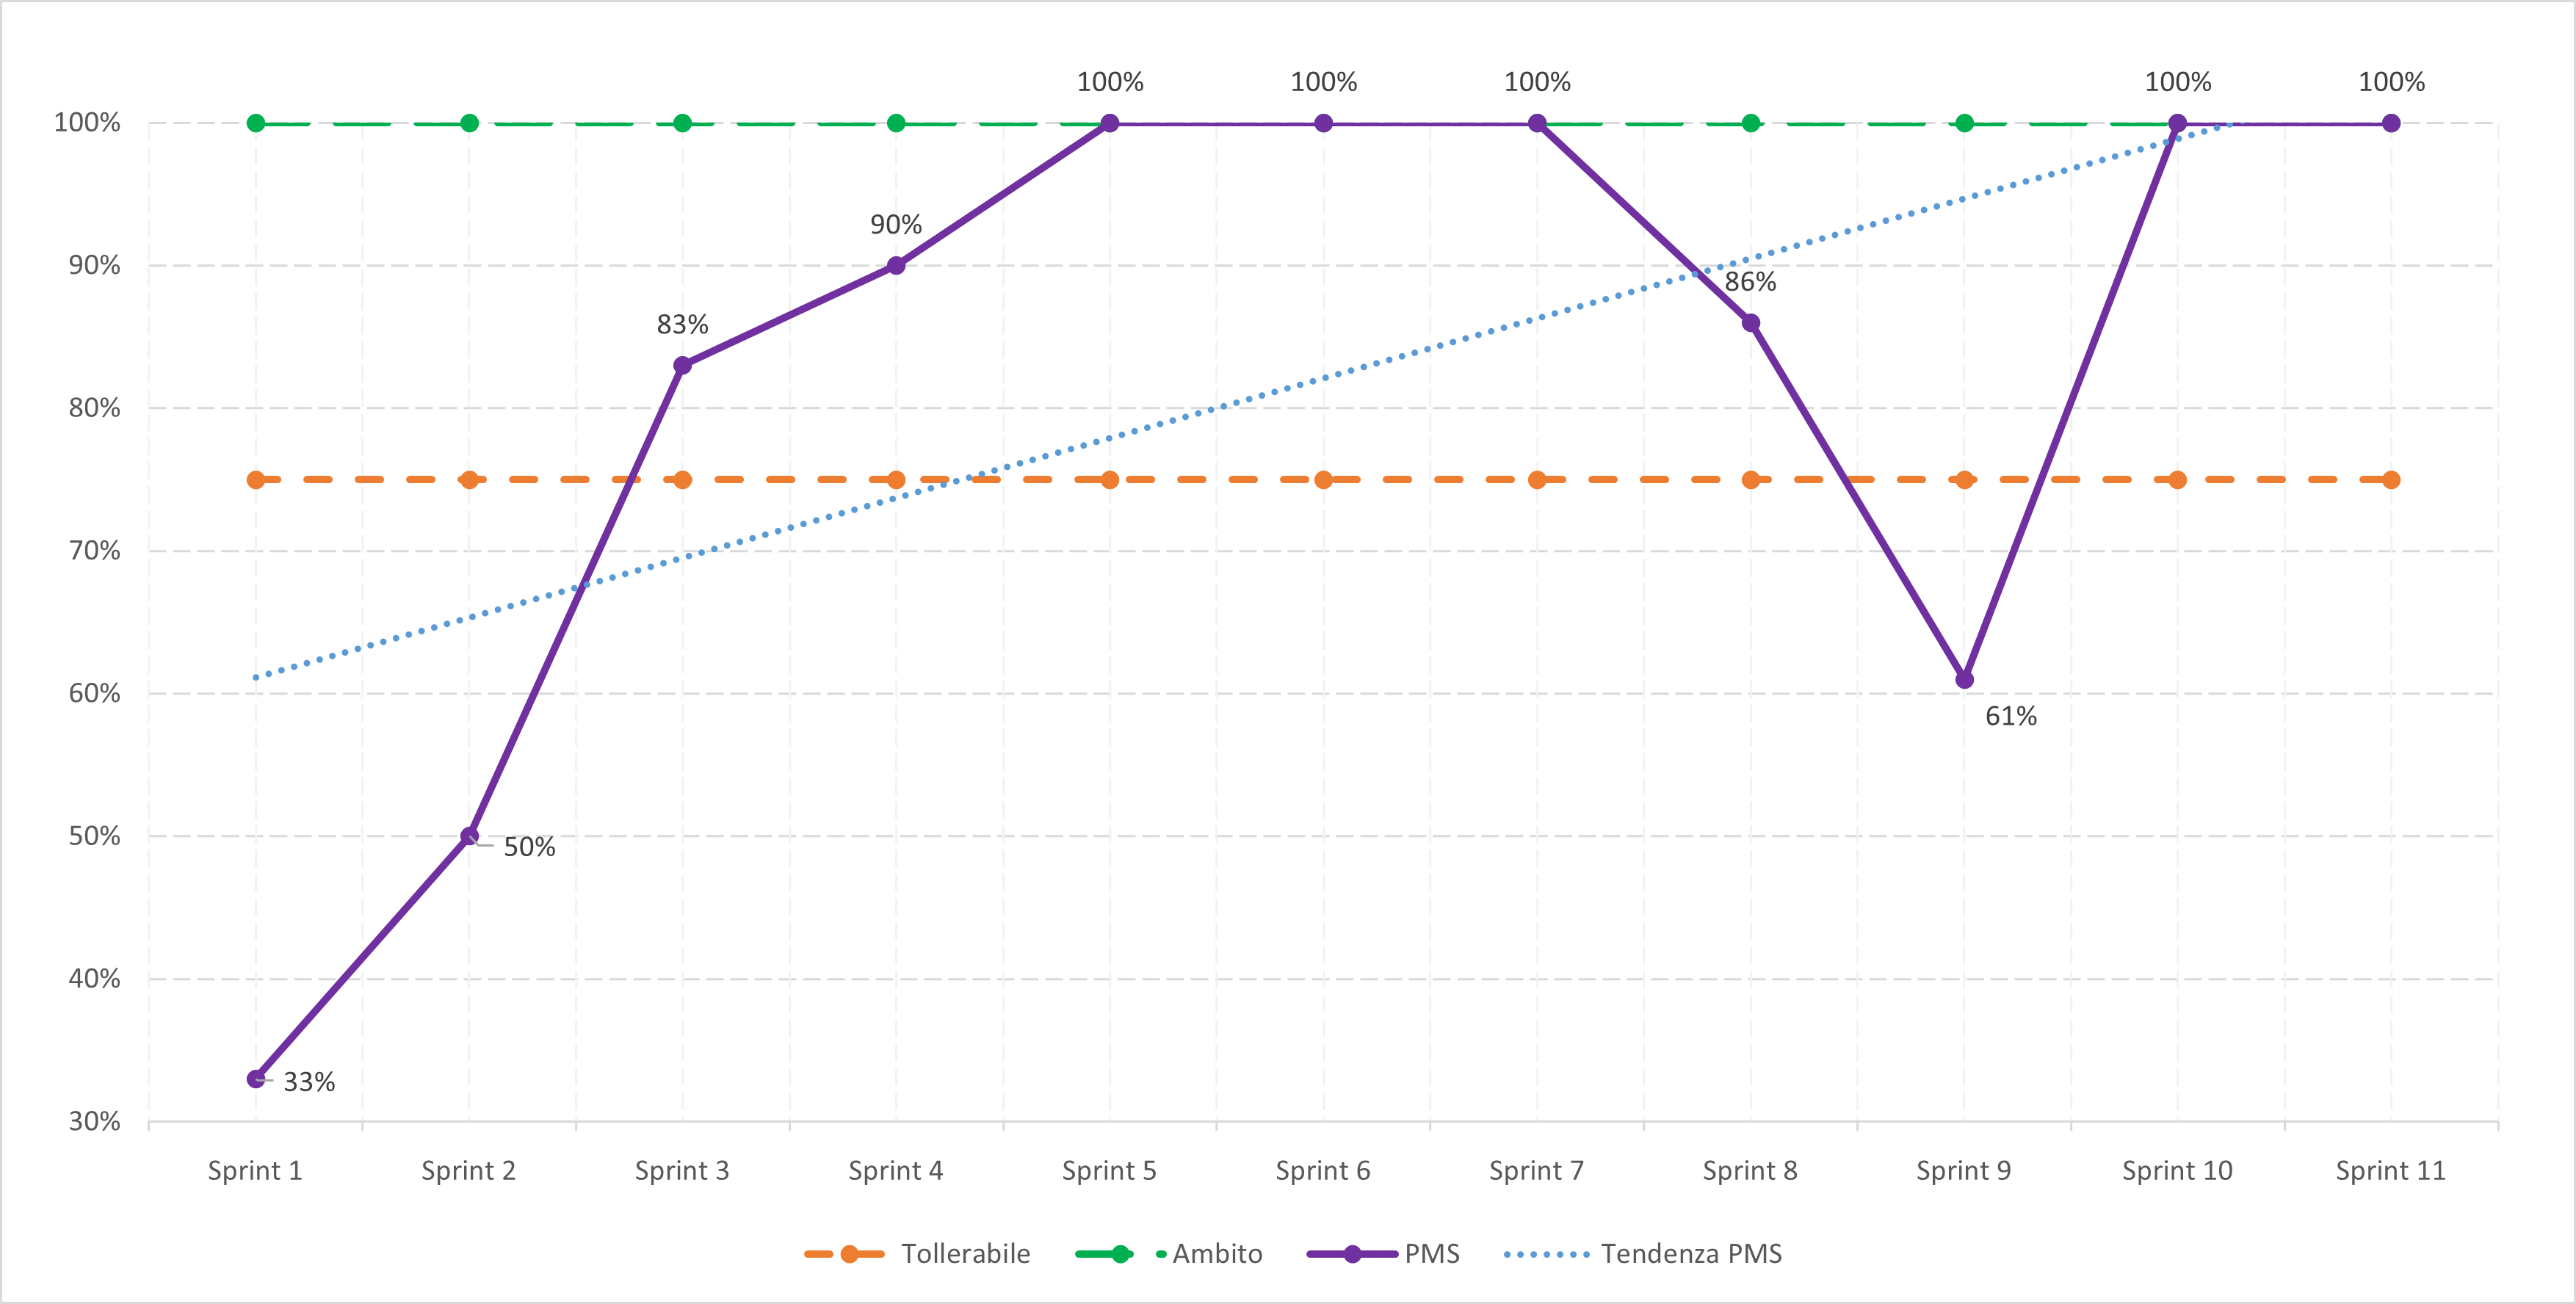
\includegraphics[width=15.5cm]{img/metriche/MPC1PMS.png}
\caption{M.PC.1.PMS - Percentuale di metriche soddisfatte.}
\end{figure}
\subsubsection{Considerazioni}
Osservando il grafico si nota come, per la maggior parte delle metriche, inizialmente non sia stata raggiunta la soglia tollerabile.
La difficoltà nel portare qualità al progetto era dovuta all’inesperienza iniziale, che ha portato il gruppo ad esplorare con cautela i vari aspetti del progetto.
Con il tempo, il team ha iniziato ad esporre più frequentemente le problematiche riscontrate, discutendo e proponendo migliorie.
Questo passo ha aiutato il gruppo a capire l’importanza della collaborazione e del dialogo aperto.
Alla fine del secondo sprint, il team ha iniziato a porre più attenzione al PDCA e alla definizione del proprio Way of working nelle Norme di progetto, aumentando notevolmente la qualità dei processi.
È possibile notare infatti un netto miglioramento a partire dal terzo sprint, fino ad arrivare ad un valore ambito, alla fine del quinto sprint. 
Il team punta a mantenere la stessa qualità anche per quanto riguarda le metriche di prodotto, le cui misurazioni verranno effettuate una volta iniziate le attività di progettazione, codifica e testing del processo di sviluppo.
\subsection{M.PC.2.RNP}
\begin{figure}[H]
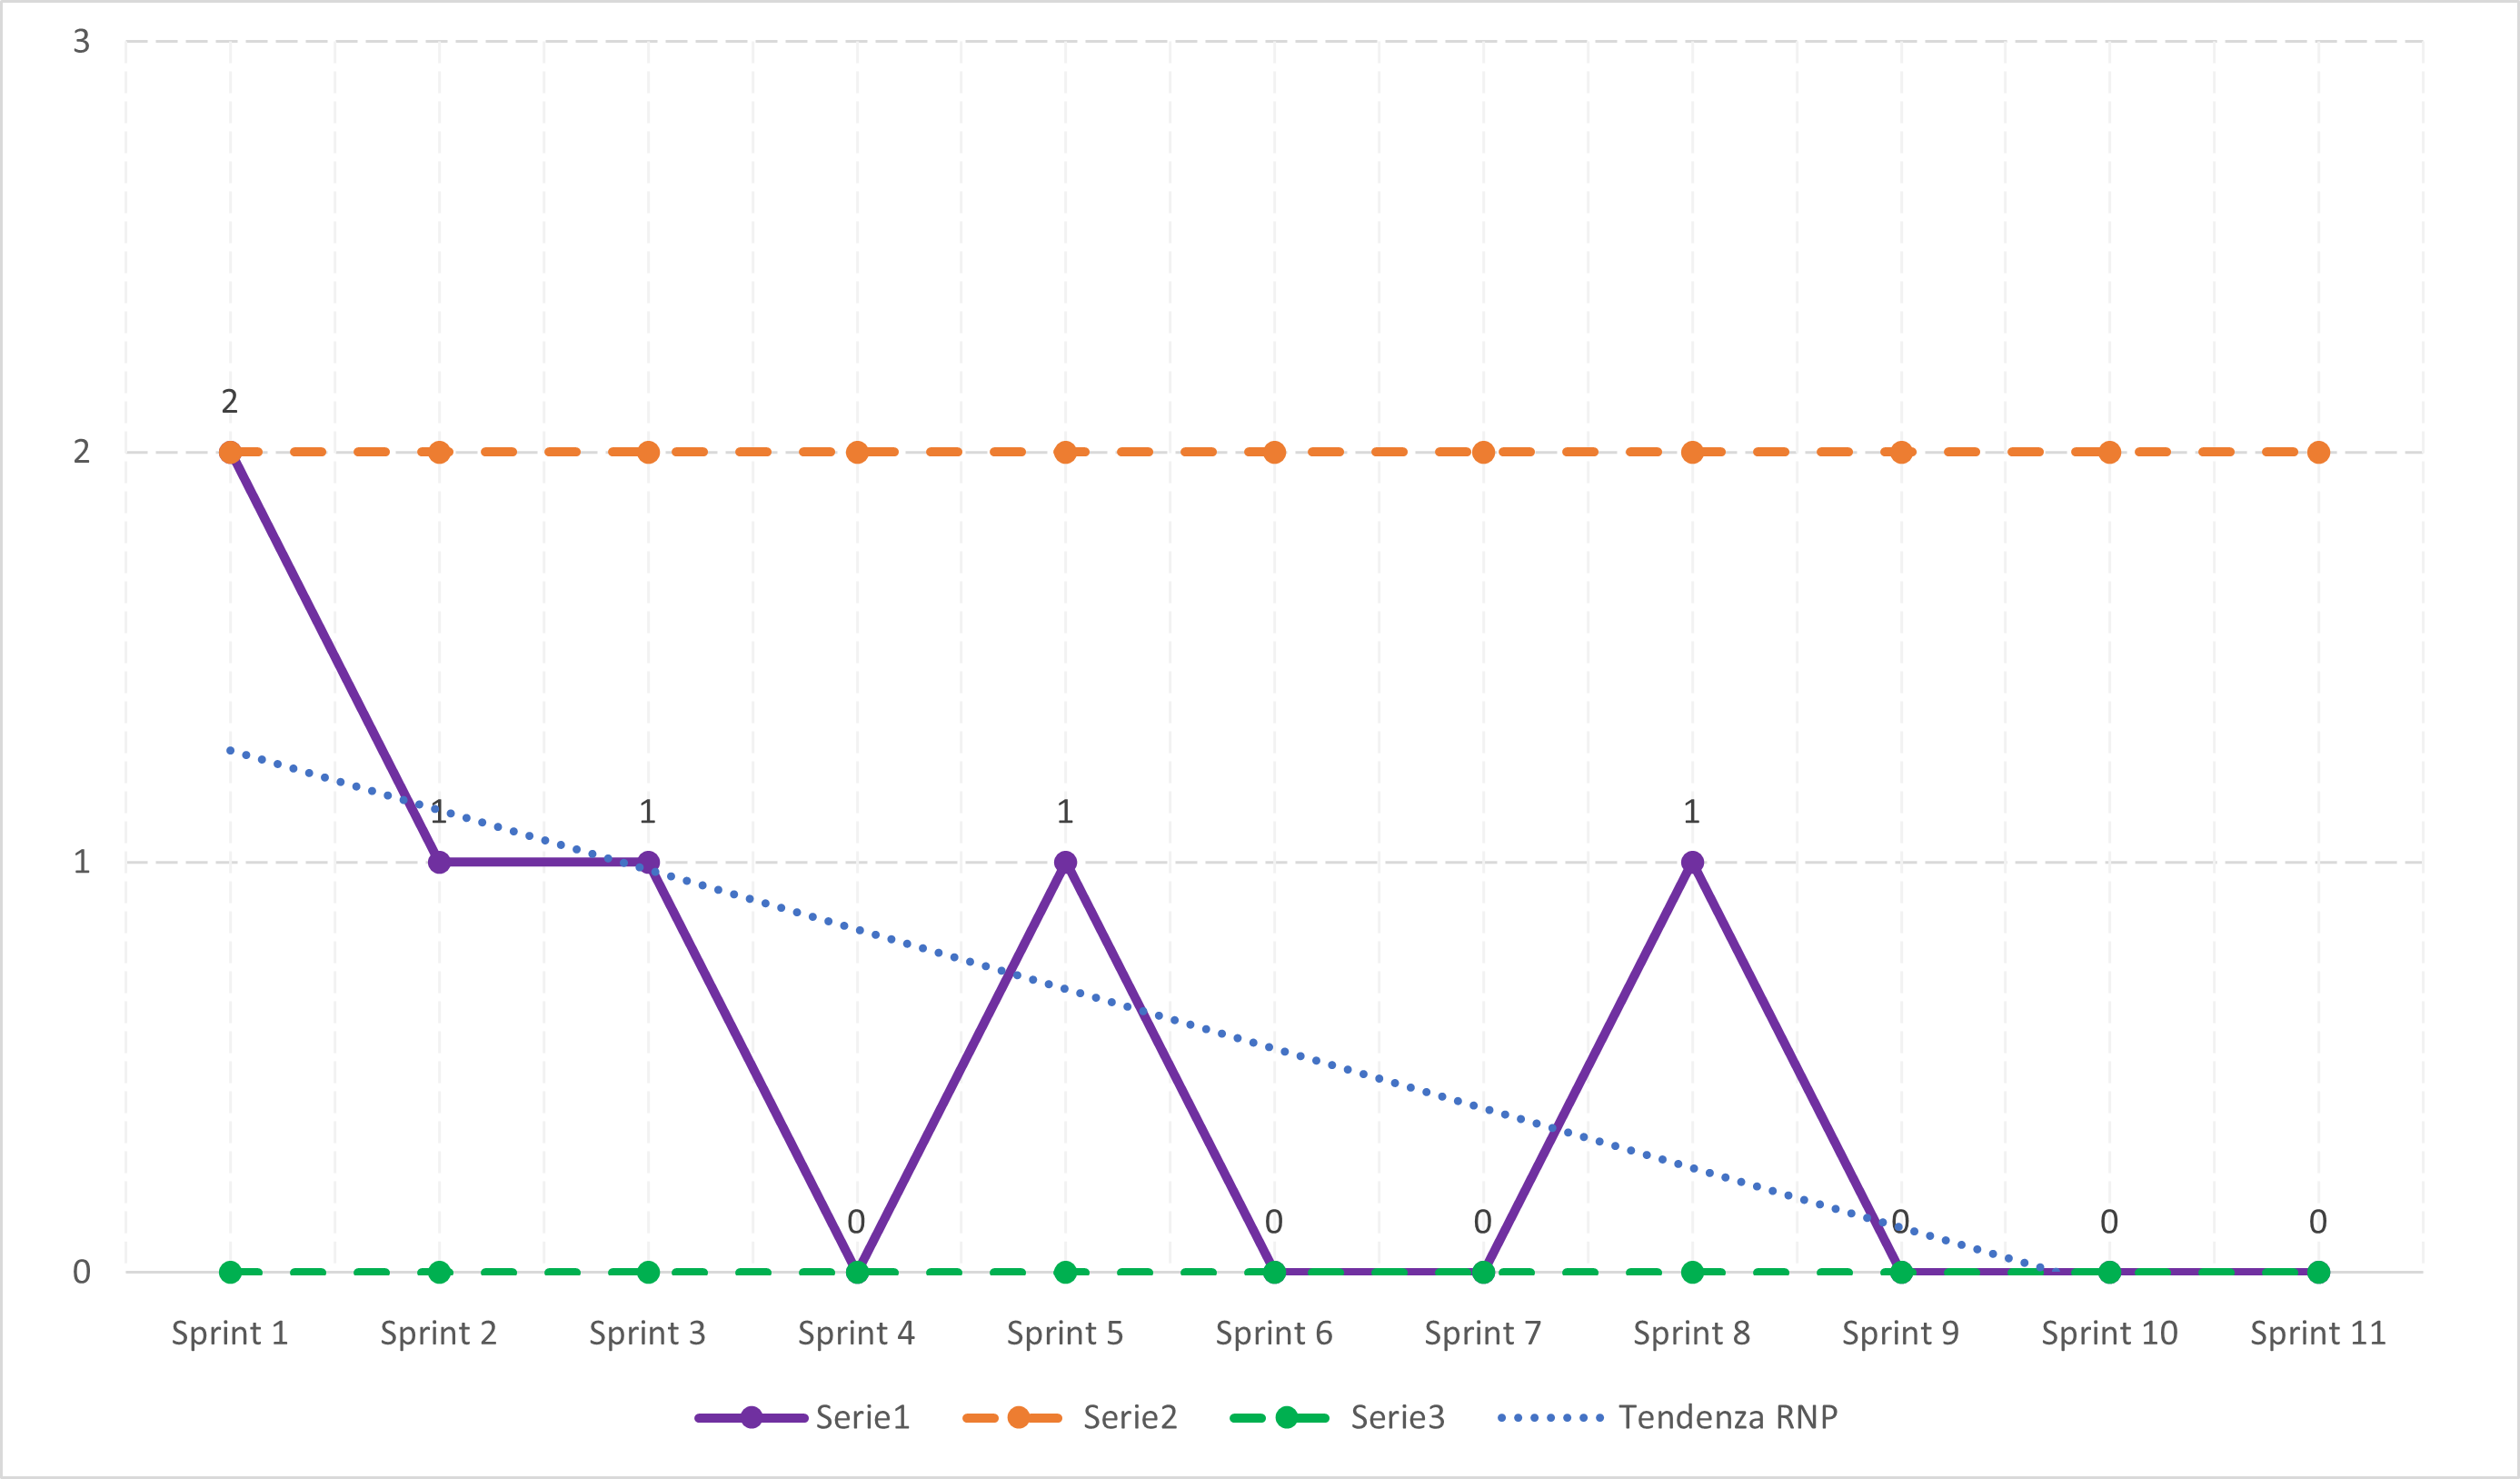
\includegraphics[width=15.5cm]{img/metriche/MPC2RNP.png}
\caption{M.PC.2.RNP - Rischi non previsti.}
\end{figure}
\subsubsection{Considerazioni}
Attraverso il grafico possiamo notare un'iniziale difficoltà nell'individuare i possibili rischi.
Si sono infatti presentati due imprevisti che sono emersi a causa della nostra inesperienza generale.
Tuttavia, il team è riuscito a mantenere la misurazione entro i limiti di tolleranza, gestendo i rischi pervenuti con metodo e ragionamento.
Nel quarto sprint non è stato riscontrato alcun rischio, raggiungendo così il livello desiderato.
Nel quinto sprint il team ha incontrato una nuova problematica legata alla scarsa comunicazione tra i membri, dovuta a impegni extra-universitari e periodi festivi.
In linea di massima, il team ha quindi inizialmente sottovalutato i rischi, imparando poi ad affrontarli in modo più professionale, riportandoli e tracciandoli in modo dettagliato attraverso discussioni documentate nei vari verbali.
\subsection{M.PC.3.VP}
\begin{figure}[H]
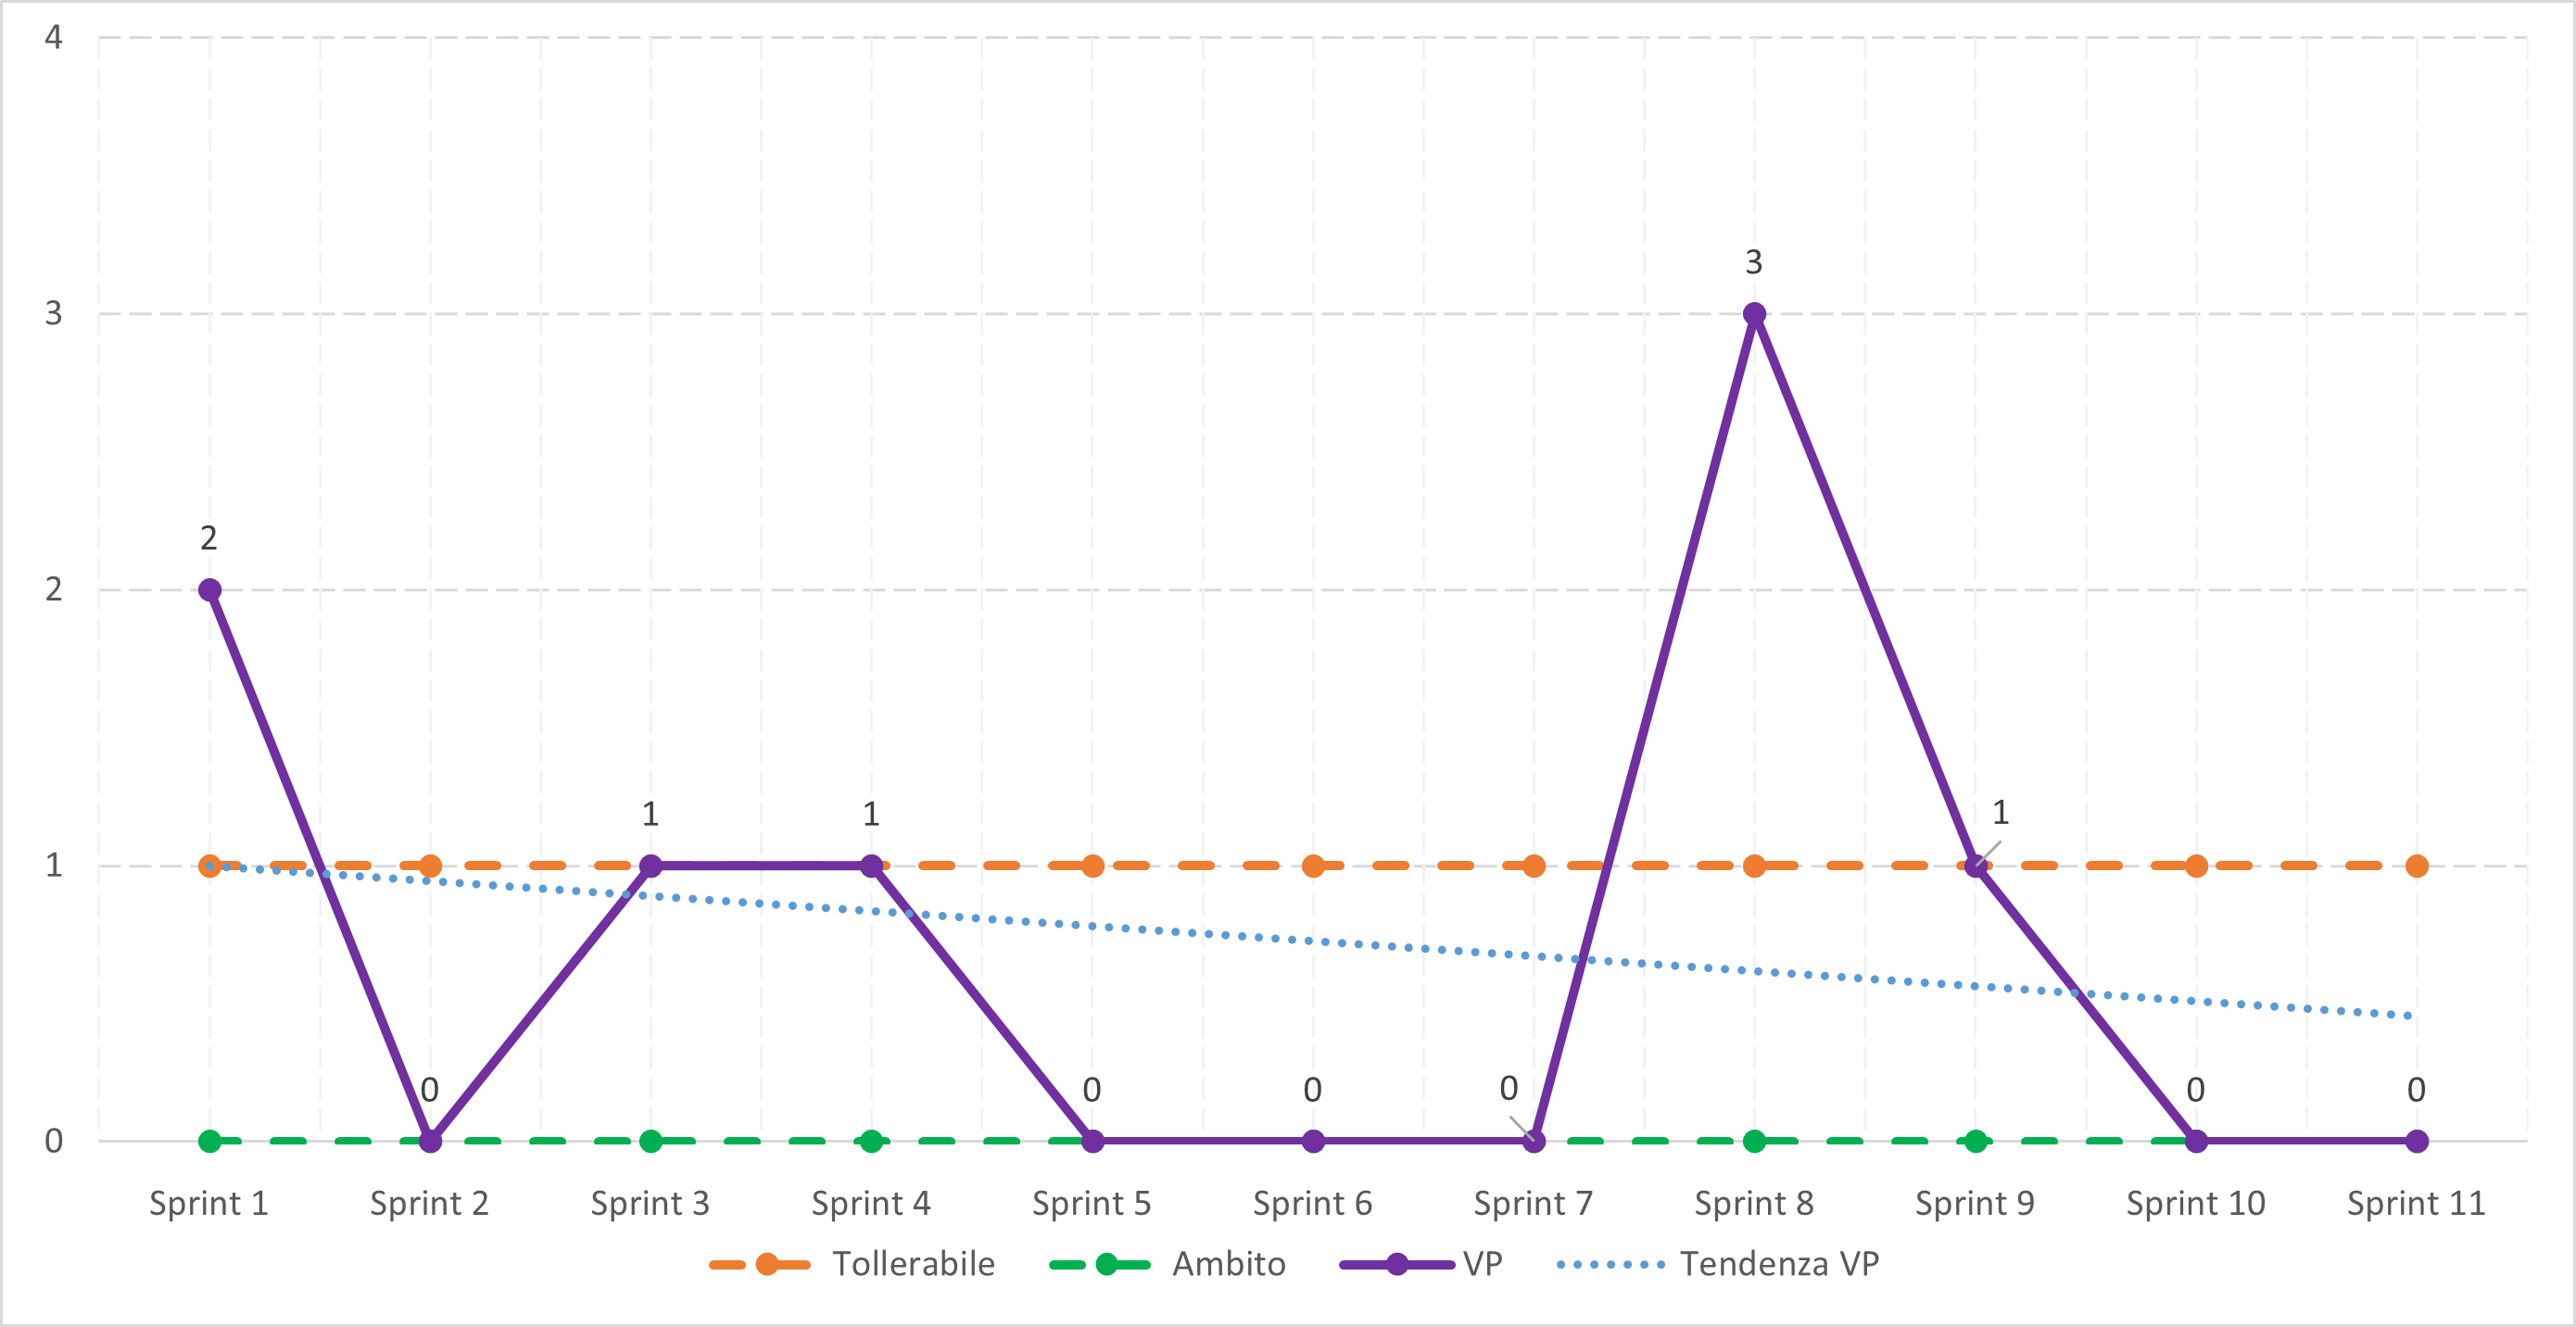
\includegraphics[width=15.5cm]{img/metriche/MPC3VP.png}
\caption{M.PC.3.VP - Variazione di piano.}
\end{figure}
\subsubsection{Considerazioni}
Inizialmente il team ha avuto difficoltà nel mantenere un ritmo adeguato e una pianificazione accurata.
A causa di una sovraccarico della quantità di lavoro assegnata ad ogni membro e di una pianificazione superficiale, si è verificata una discrepanza significativa tra i compiti pianificati e quelli effettivamente completati.
Tuttavia, nel secondo sprint, il team ha preso decisioni più precise e prudenti, raggiungendo un livello ottimale di performance.
Successivamente, dopo due sprint con un leggero technical debt legato alla grande quantità di lavoro pianificato, il team è riuscito a ristabilire il valore ambito durante il quinto e sesto sprint.
\subsection{M.PC.4.VC}
\begin{figure}[H]
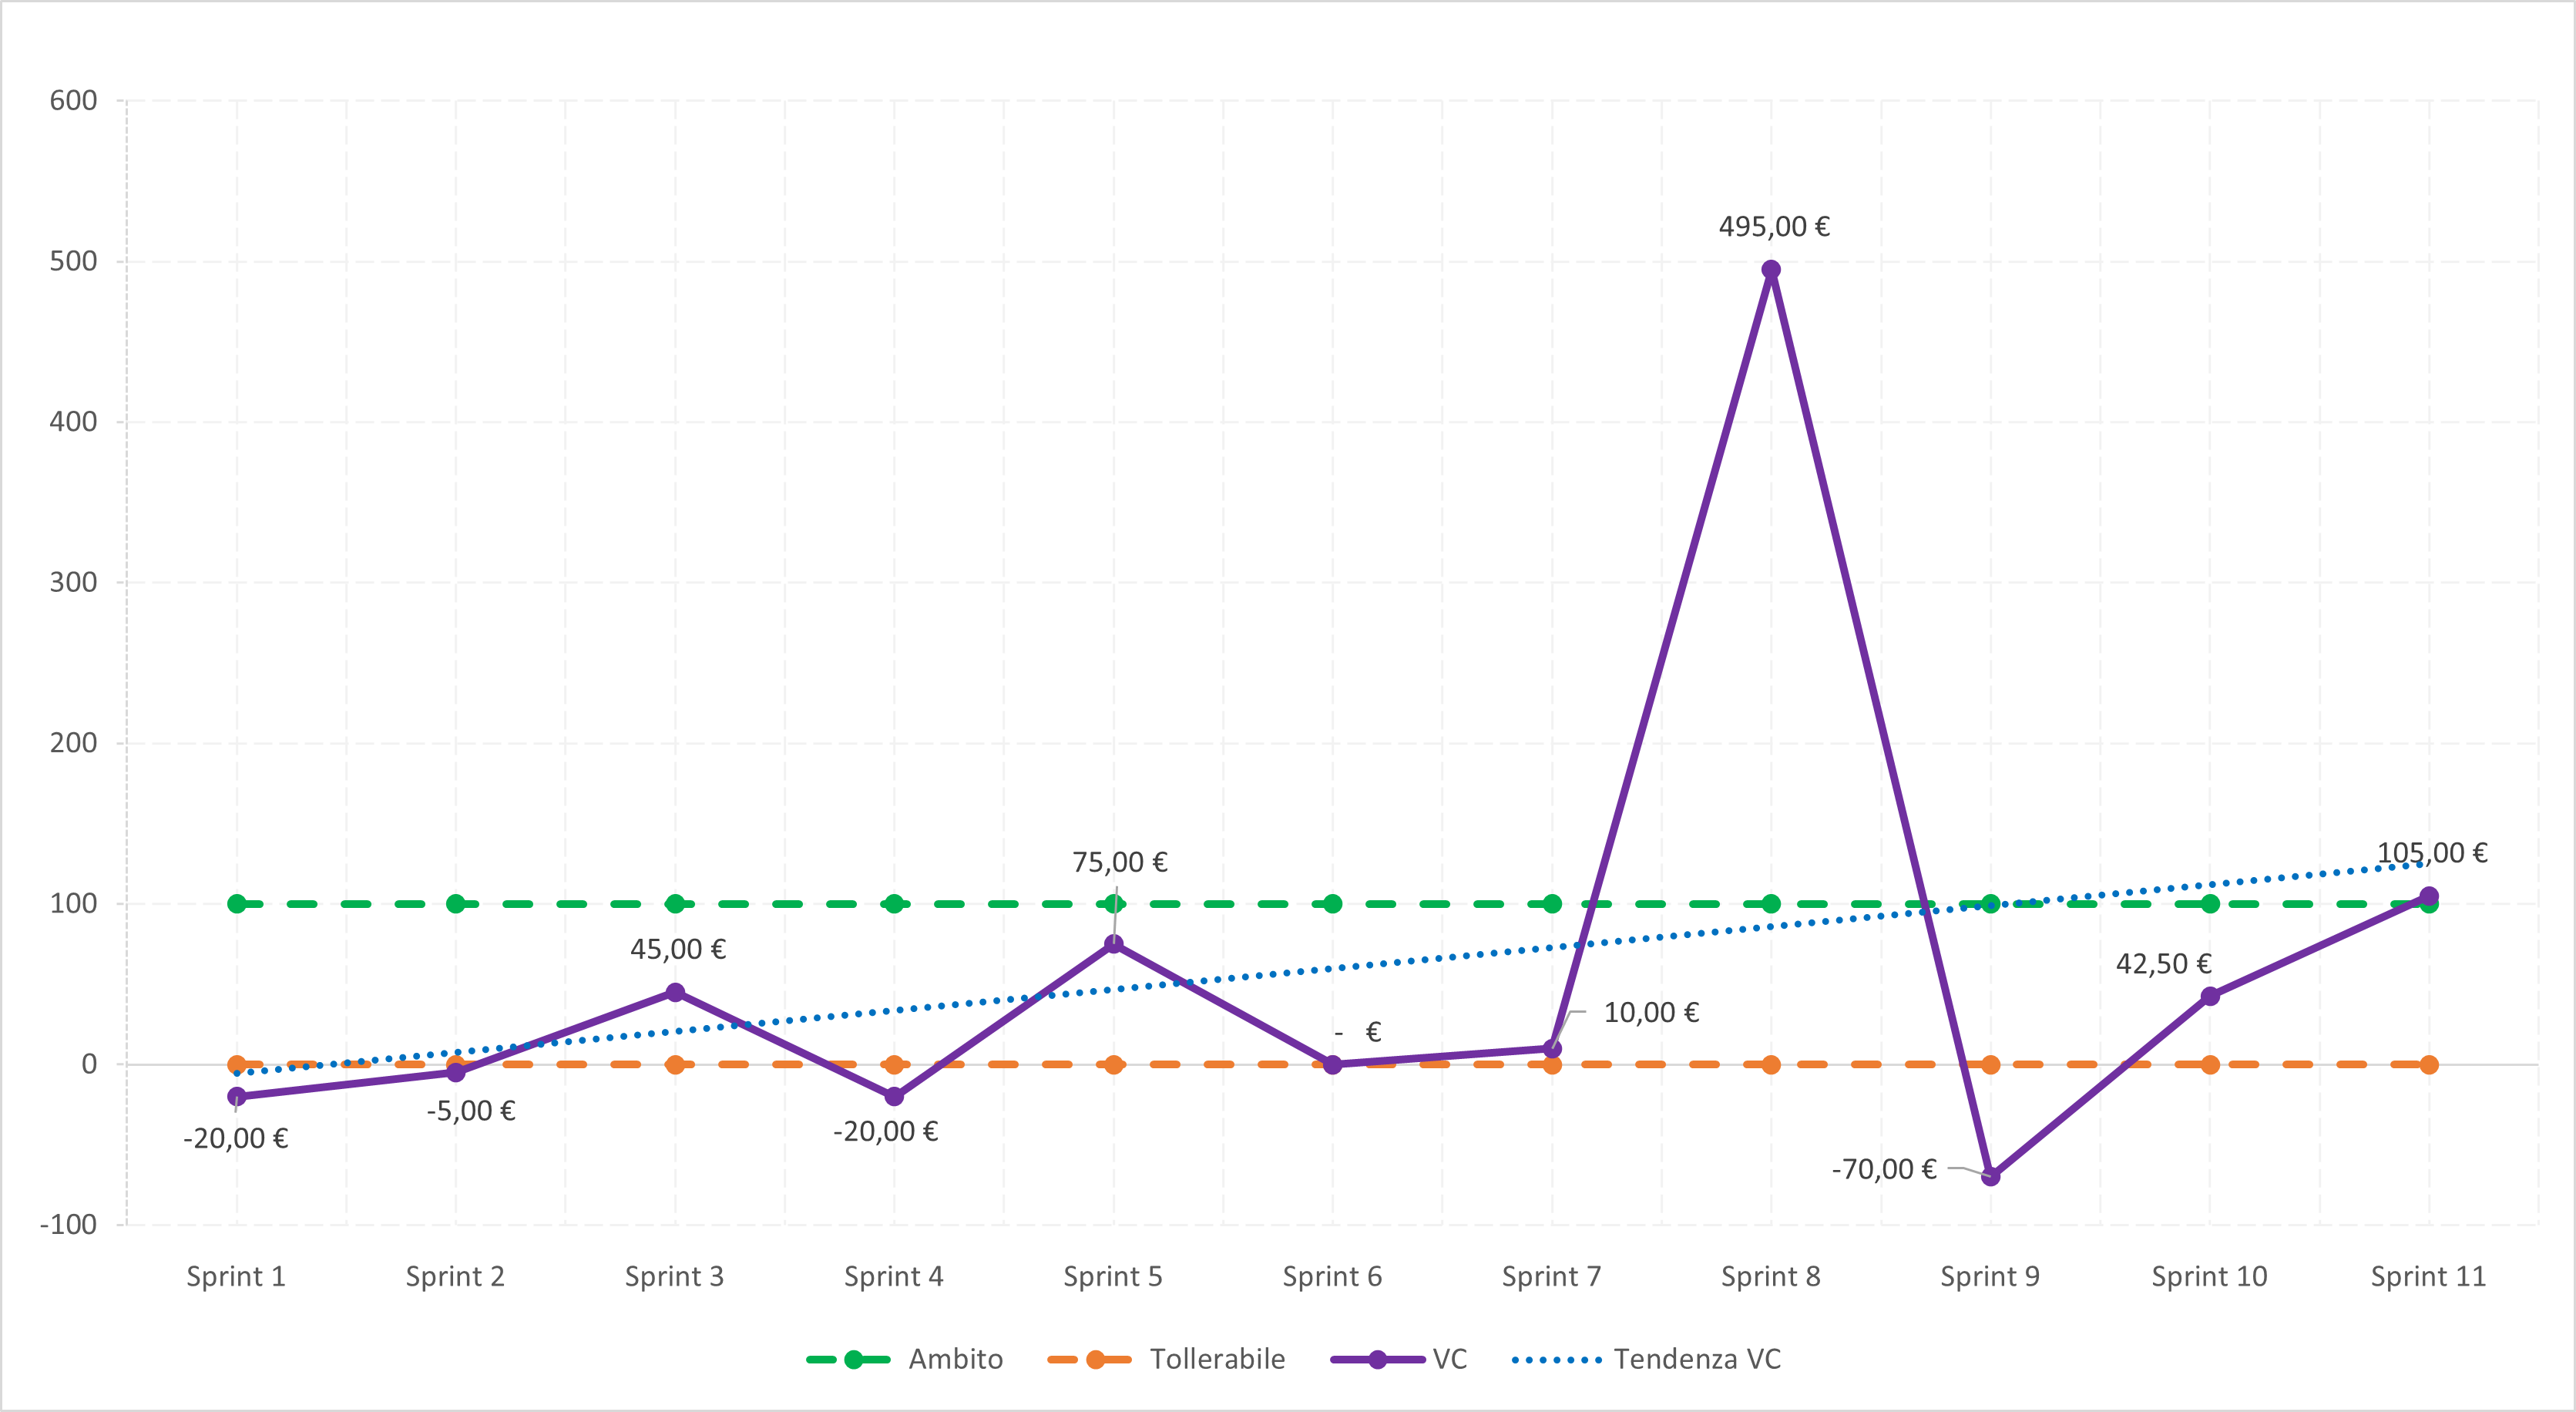
\includegraphics[width=15.5cm]{img/metriche/MPC4VC.png}
\caption{M.PC.4.VC - Variazione di costo.}
\end{figure}
\subsubsection{Considerazioni}
Inizialmente il team ha sottovalutato la quantità di lavoro necessario per completare le attività pianificate, superando i costi stimati.
Nel terzo periodo, data una sovrastima dei costi di realizzazione del PoC, il team è riuscito a contenere le spese e rientrare nelle stime iniziali.
Durante il quarto sprint, il colloquio con il professor Cardin ha richiesto una ristrutturazione dell'Analisi dei requisiti, causando un aumento delle ore dedicate alla preparazione della prima revisione RTB.
Nonostante questo impegno aggiuntivo e apparentemente dispendioso, il team è riuscito a portare a termine lo sprint limitando le perdite.
Il gruppo punta a migliorare la pianificazione, ponendo più attenzione alla definizione dei task e alla loro stima oraria, cercando di abbassare la varianza, molto evidente nel grafico. 
\subsection{M.PC.5.ISR}
\begin{figure}[H]
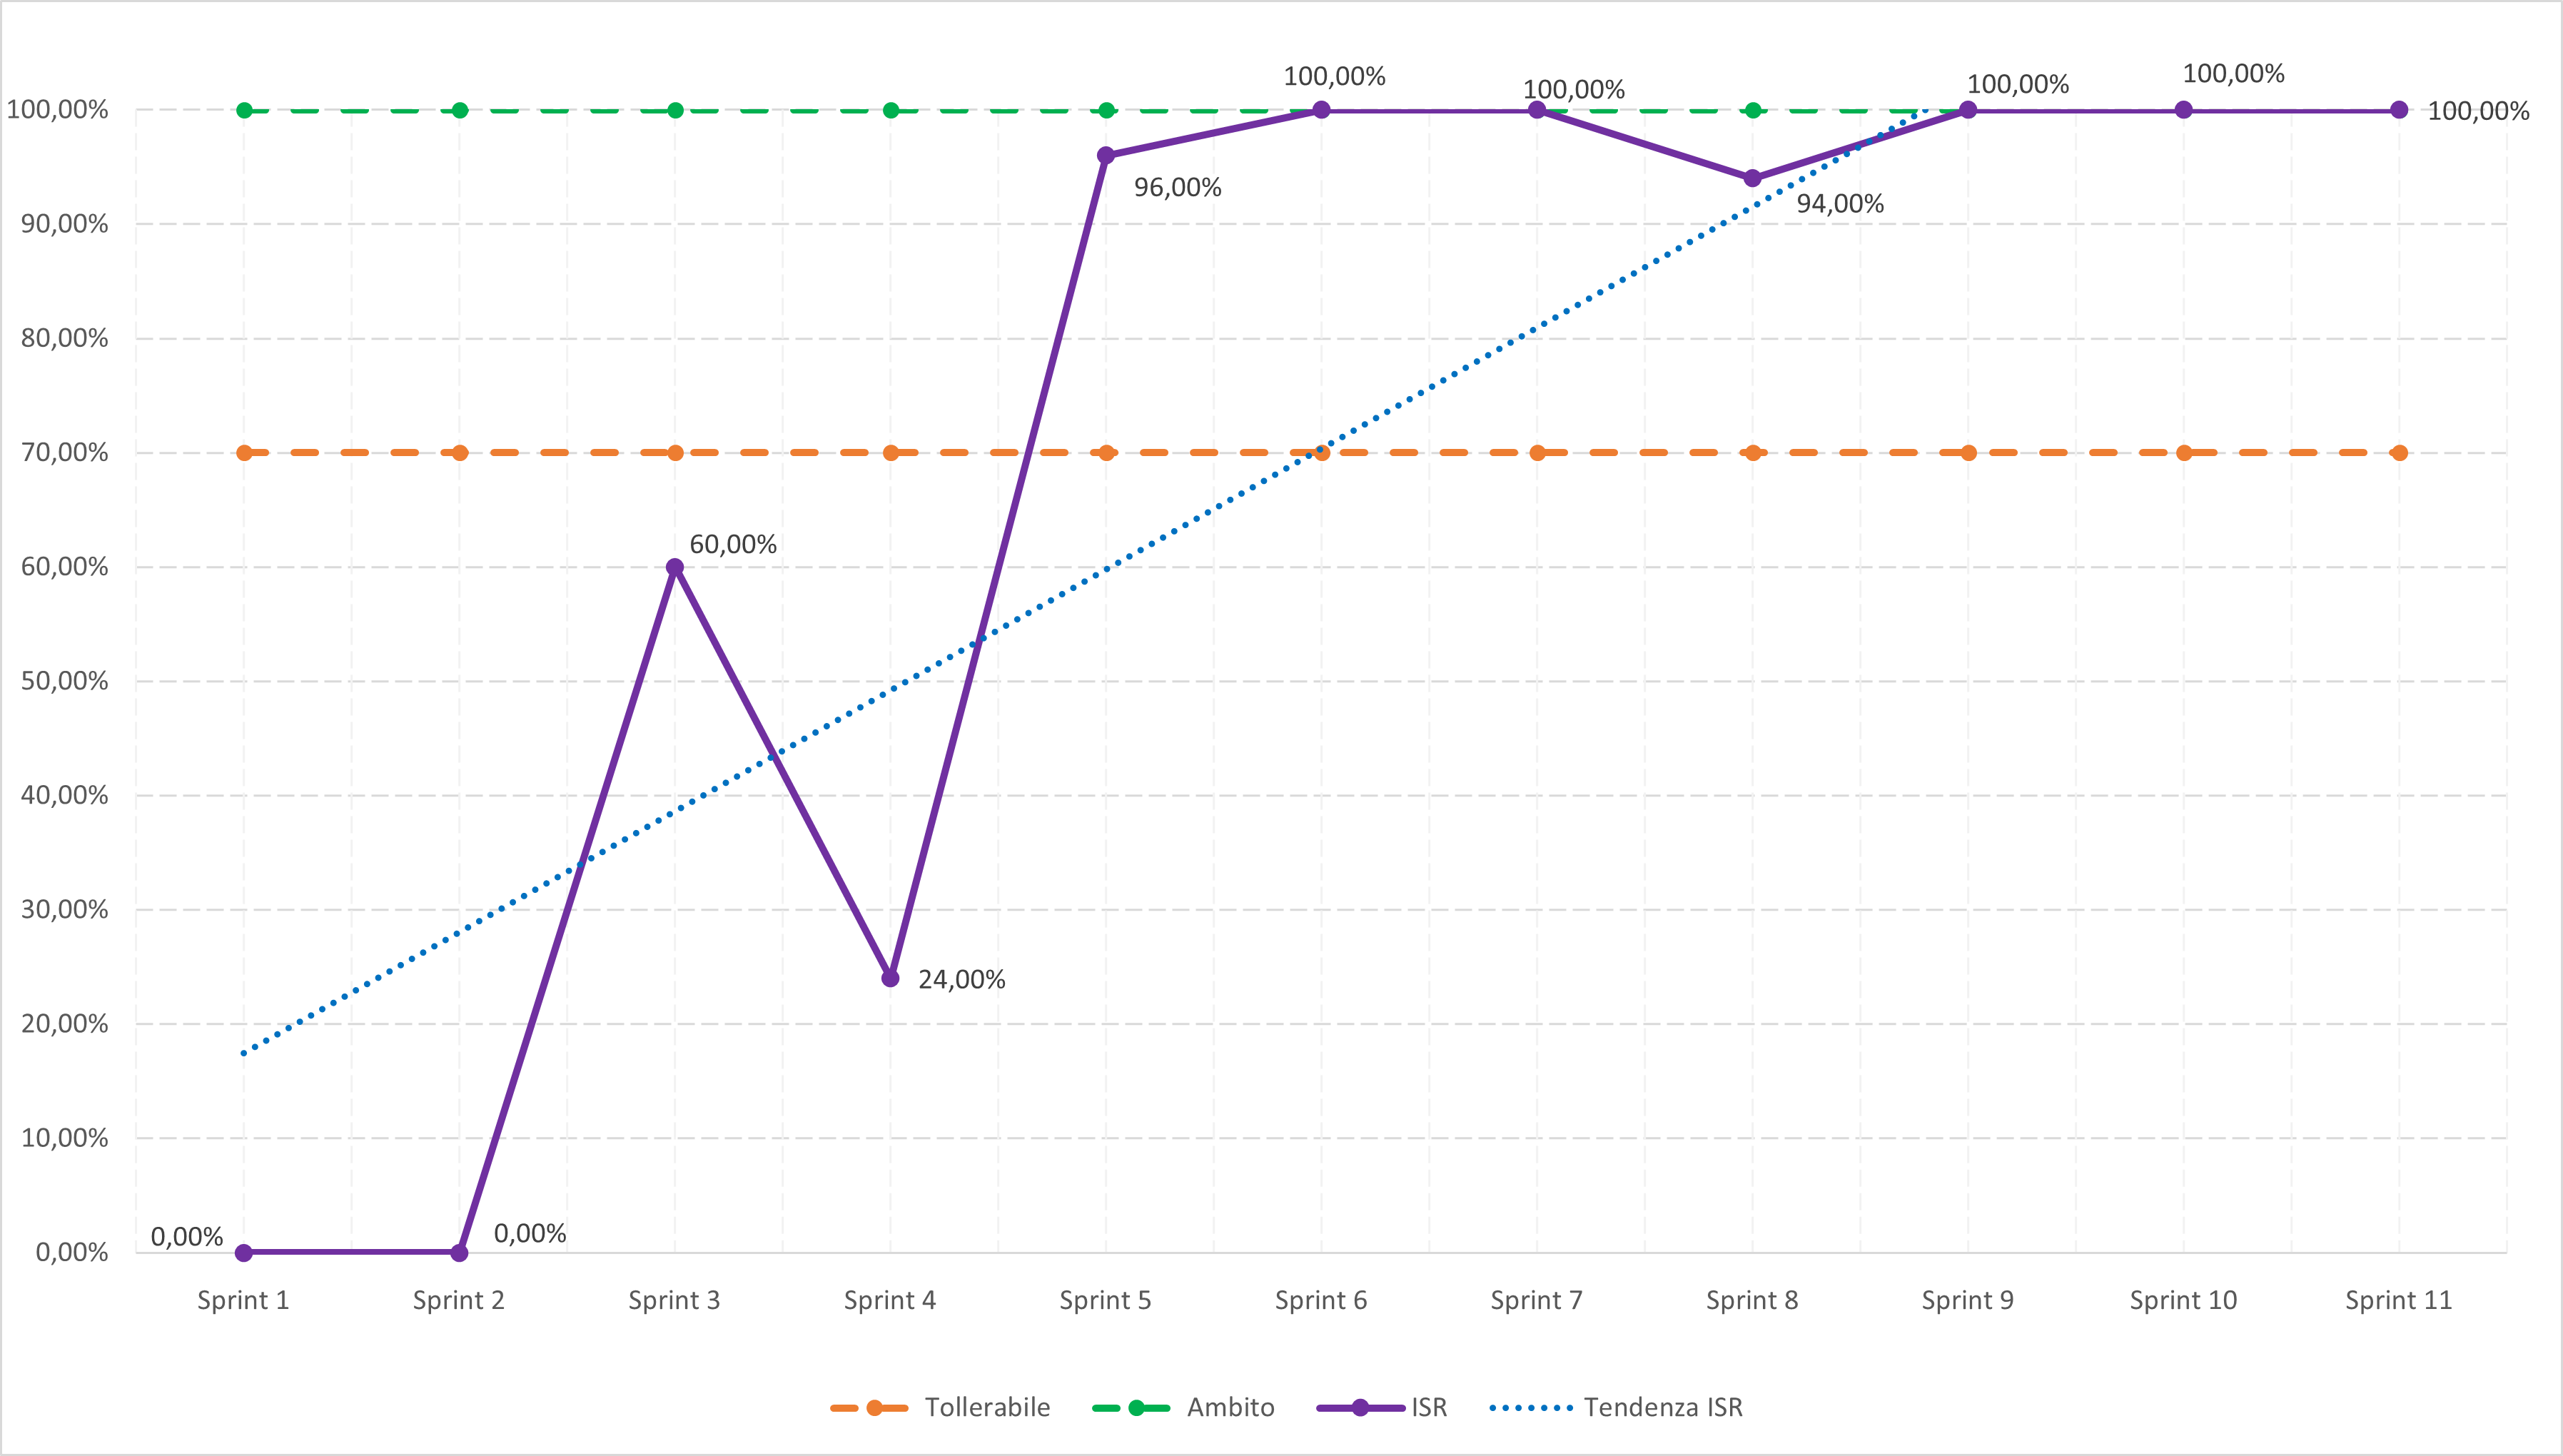
\includegraphics[width=15.5cm]{img/metriche/MPC5ISR.png}
\caption{M.PC.5.ISR - Indice di stabilità dei requisiti.}
\end{figure}
\subsubsection{Considerazioni}
Nei primi due sprint, la nostra inesperienza nella definizione di un gran numero di requisiti ha portato ad un'alta instabilità dei requisiti.
Nel terzo sprint, il team ha aggiunto numerosi requisiti, anche grazie a incontri interni ed esterni che hanno contribuito a rendere più chiare le funzionalità del prodotto.
Nel quarto sprint, dopo un incontro con il Professore Cardin, è stato necessario ristrutturare l'Analisi dei requisiti, sia per struttura del documento che per contenuto.
Nel quinto e sesto sprint, il team ha rapidamente ristabilito l'ordine, definendo un elenco dei requisiti che, al netto di eventuali modifiche future limitate, rappresenterà l'insieme finale che verrà considerato nello sviluppo dell'MVP.
\subsection{M.PC.6.CCM}
Questa metrica verrà misurata solo dopo il superamento della revisione RTB.
\subsection{M.PC.7.SC}
Questa metrica verrà misurata solo dopo il superamento della revisione RTB.
\subsection{M.PC.8.BC}
Questa metrica verrà misurata solo dopo il superamento della revisione RTB.
\subsection{M.PC.9.ET}
\begin{figure}[H]
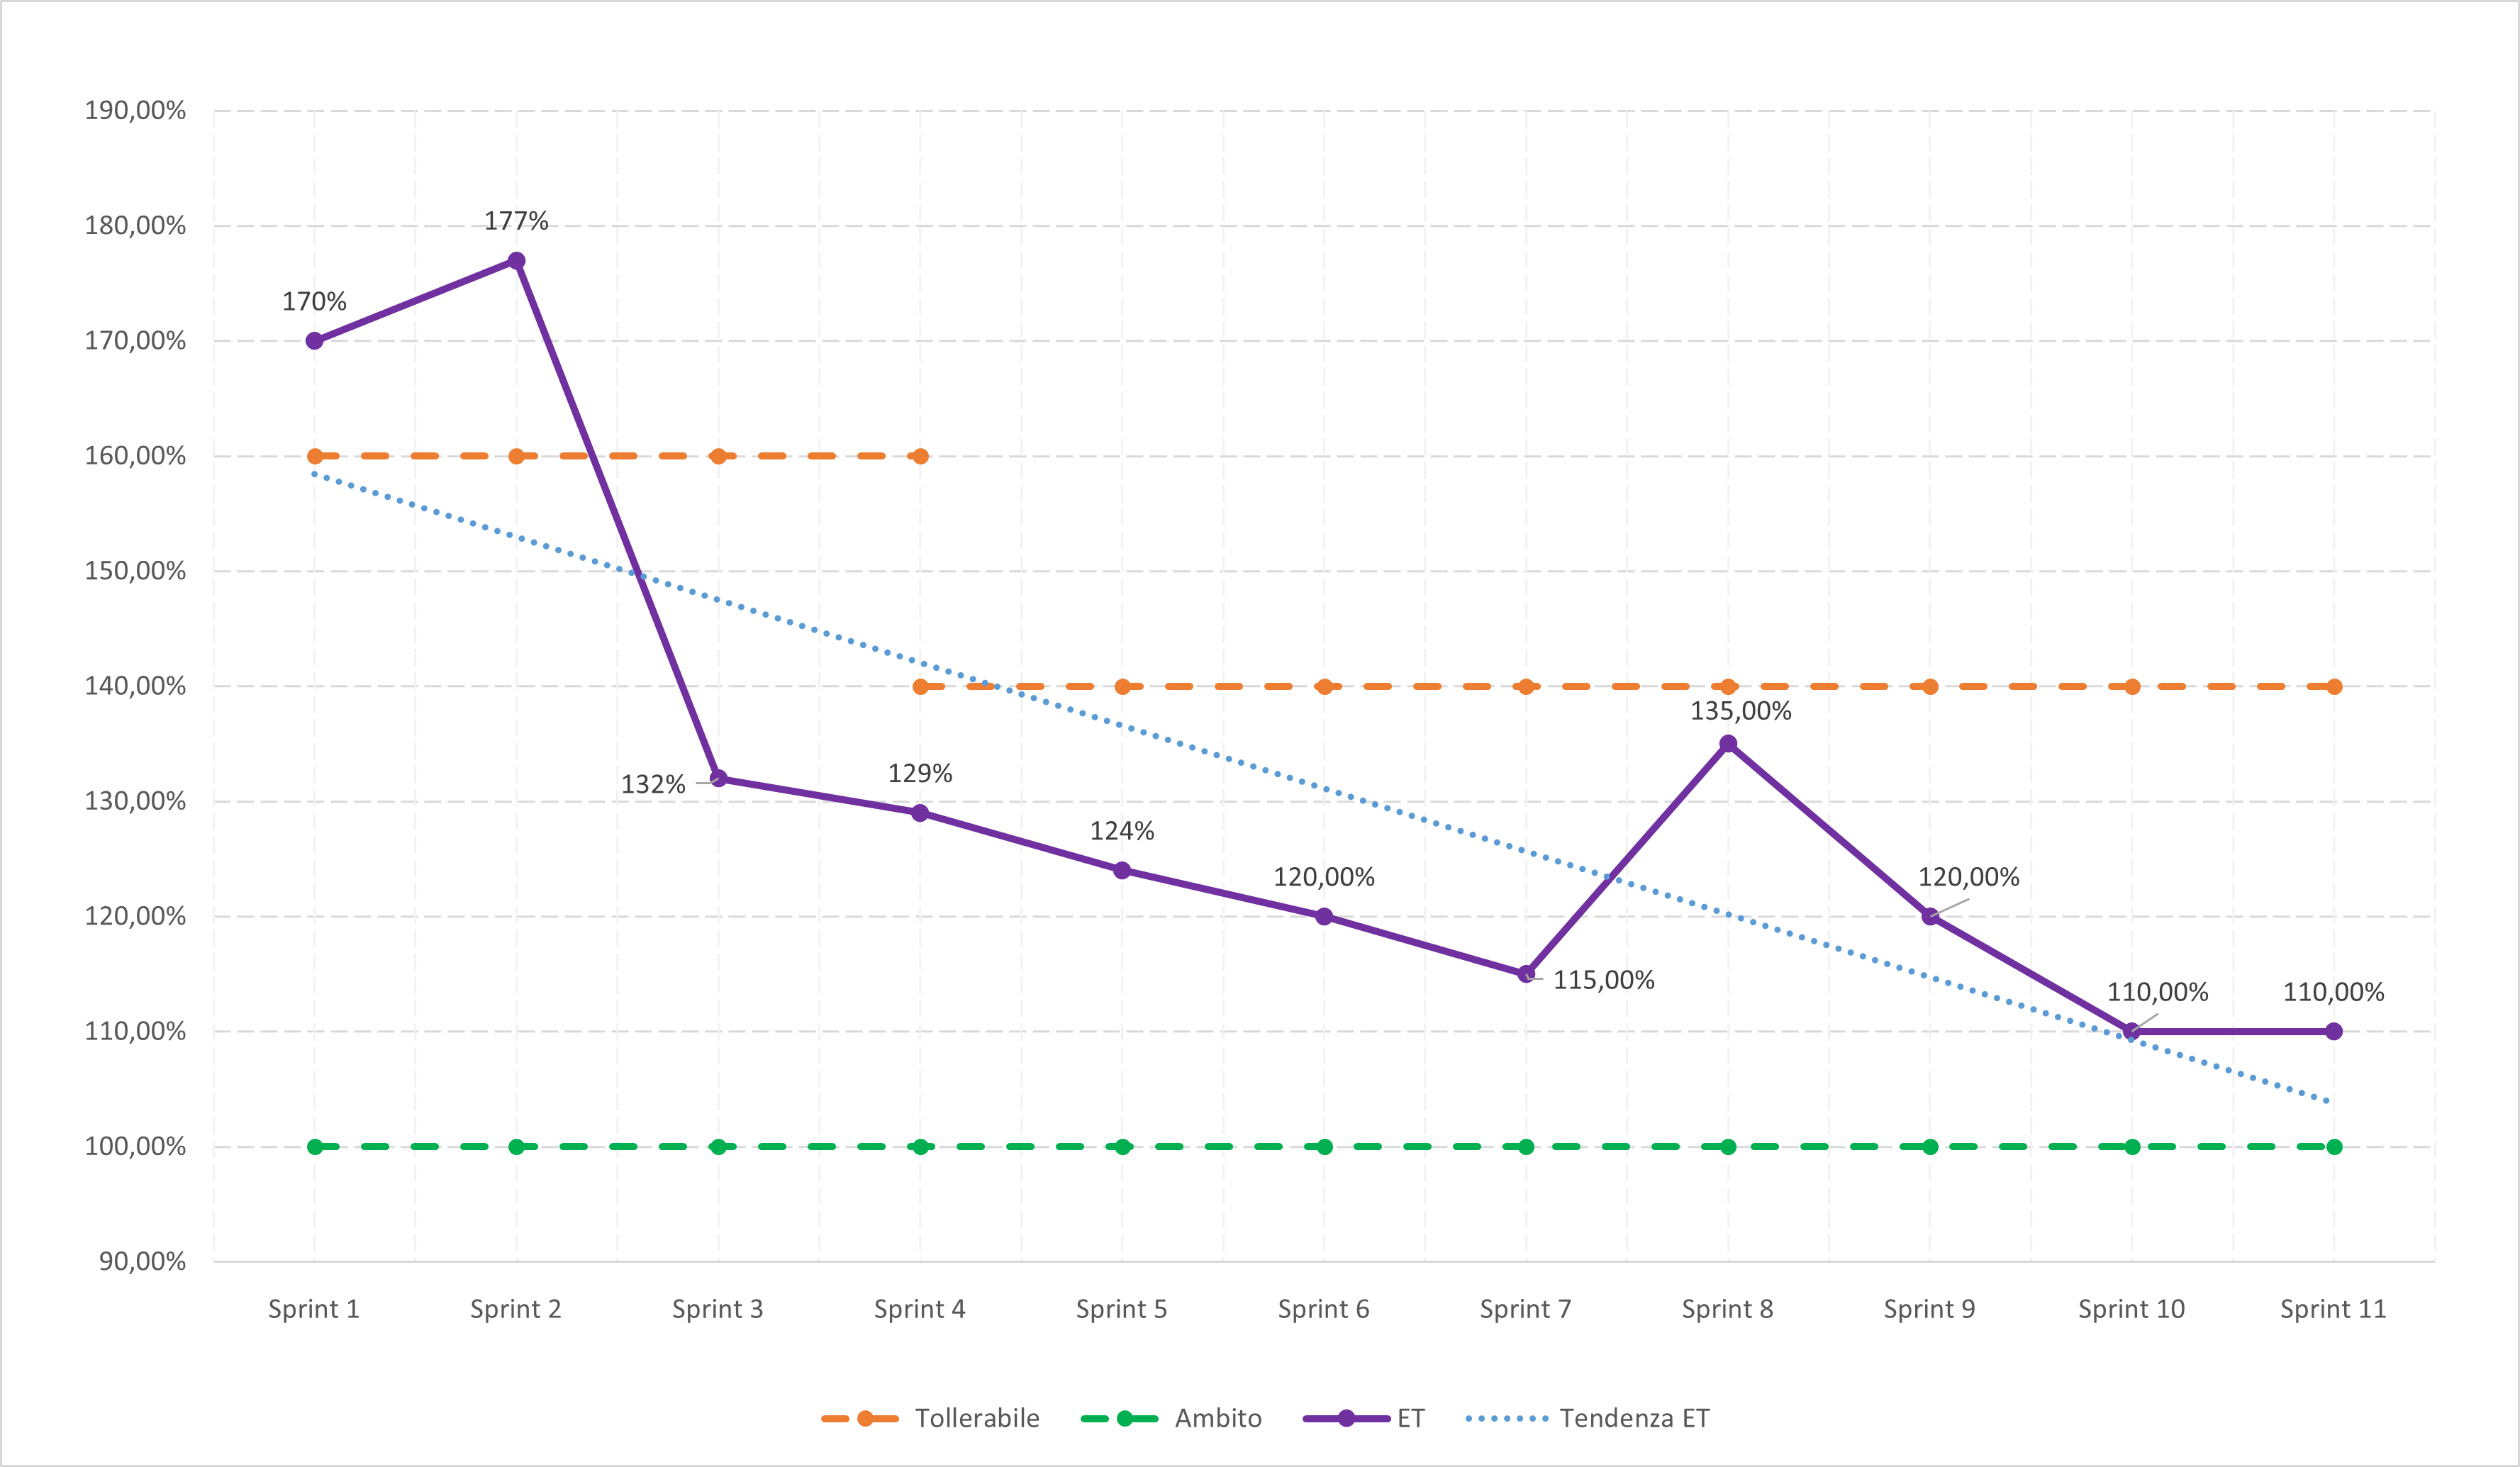
\includegraphics[width=15.5cm]{img/metriche/MPC9ET.png}
\caption{M.PC.9.ET - Efficienza temporale.}
\end{figure}
\subsubsection{Considerazioni}
Nonostante un inizio caratterizzato da un elevato rapporto tra ore di lavoro e ore produttive, dovuto all'inesperienza e alla scarsa familiarità con gli strumenti utilizzati, si è registrato un notevole miglioramento dal terzo sprint in poi.
Questo è stato possibile grazie al miglioramento delle norme, che hanno infatti ricoperto la funzione di guida durante lo svolgimento delle attività da parte dei componenti del gruppo.
Con l'obiettivo di migliorare in modo costante la qualità, il team ha deciso di ridurre la soglia tollerabile da 160\% a 140\%.
Il team punta a migliorare ulteriormente questo rapporto, ritenendolo uno degli indicatori più importanti da considerare nella valutazione dell'automiglioramento.
\subsection{M.PD.1.IG}
\begin{figure}[H]
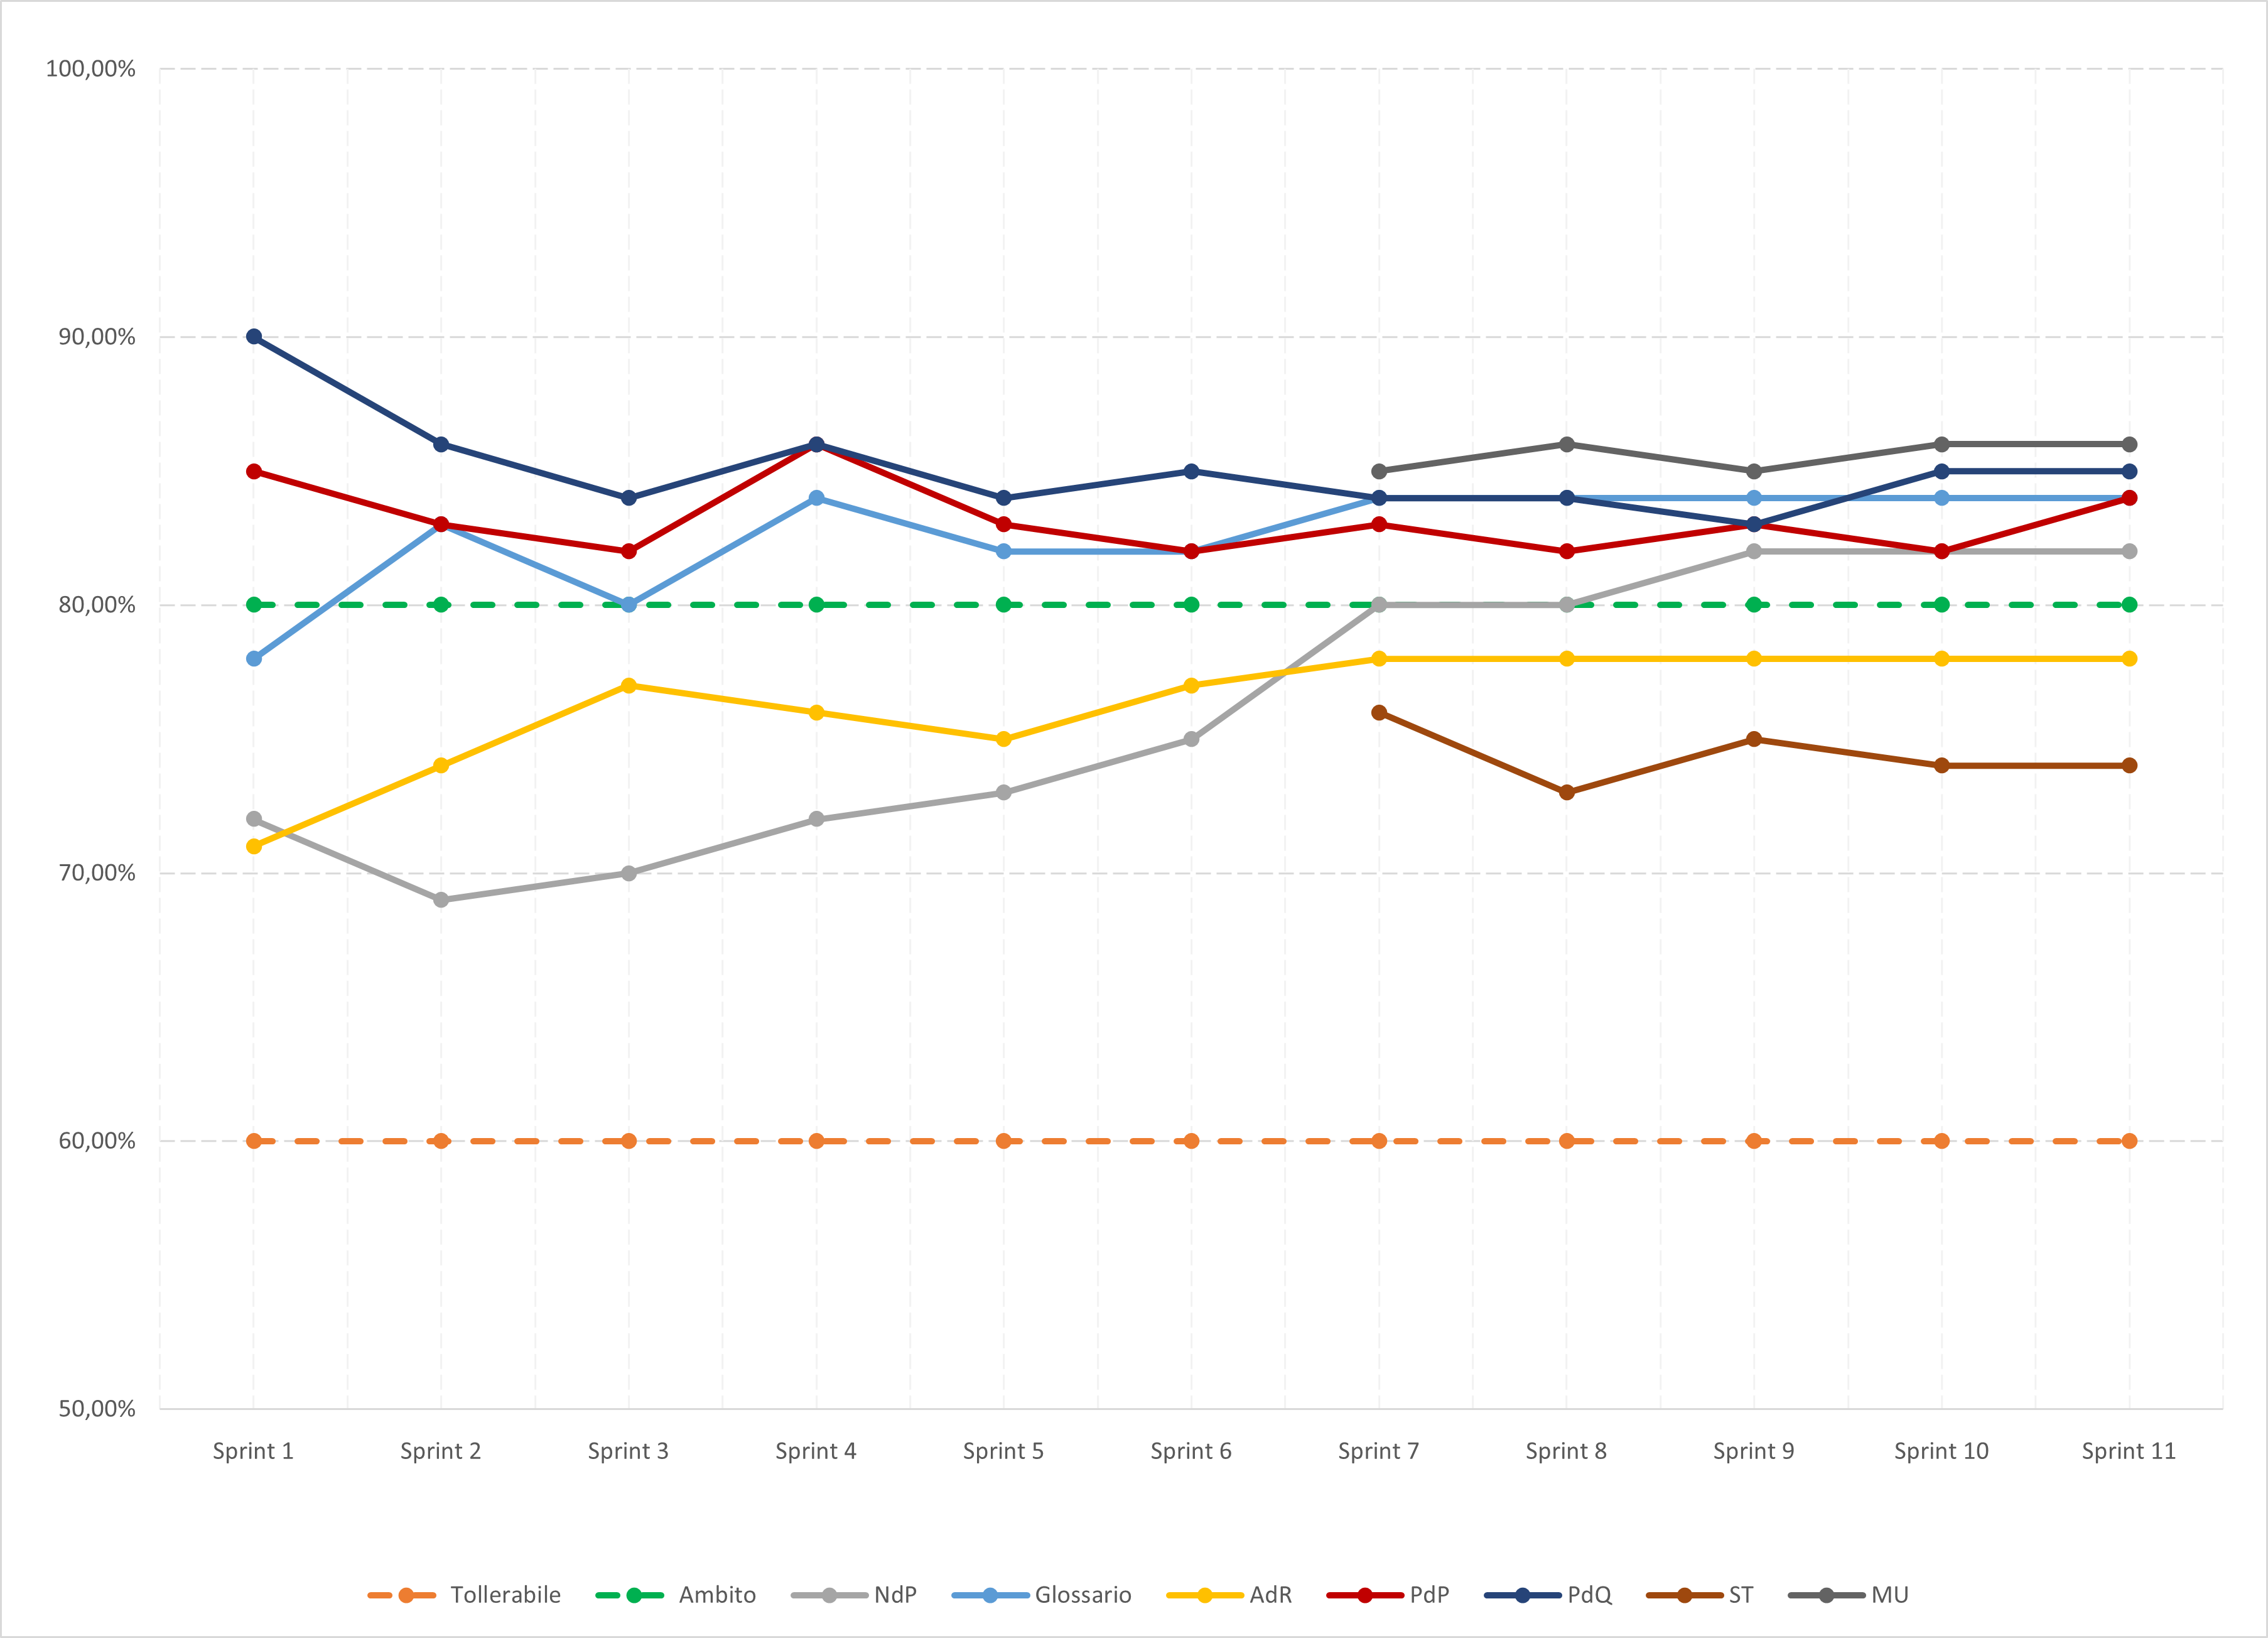
\includegraphics[width=15.5cm]{img/metriche/MPD1IG.png}
\caption{M.PD.1.IG - Indice di Gulpease.}
\end{figure}
\subsubsection{Considerazioni}
Tutti i documenti sono facilmente comprensibili anche per chi ha una licenza media, poiché rispettano la soglia di tolleranza del 60\%.
Trattando argomenti più specifici, le Norme di progetto utilizzano frasi più elaborate, rendendo l'indice di leggibilità di tale documento leggermente più basso degli altri.
Il gruppo pensa di continuare a migliorare questo indice rielaborando i periodi lunghi, abbreviandoli o riformulando i concetti esposti ove possibile.
\subsection{M.PD.2.LMC}
Questa metrica verrà misurata solo dopo il superamento della revisione RTB.
\subsection{M.PD.3.AFS}
Questa metrica verrà misurata solo dopo il superamento della revisione RTB.
\subsection{M.PD.4.AR}
Questa metrica verrà misurata solo dopo il superamento della revisione RTB.
\subsection{M.PD.5.RD}
Questa metrica verrà misurata solo dopo il superamento della revisione RTB.
\subsection{M.PD.6.LCG}
Questa metrica verrà misurata solo dopo il superamento della revisione RTB.
\subsection{M.PD.7.CD}
Questa metrica verrà misurata solo dopo il superamento della revisione RTB.
\subsection{M.PD.8.IM}
Questa metrica verrà misurata solo dopo il superamento della revisione RTB.
\subsection{M.PD.9.TS}
Questa metrica verrà misurata solo dopo il superamento della revisione RTB.
\subsection{M.PD.10.CSD}
Questa metrica verrà misurata solo dopo il superamento della revisione RTB.
\subsection{M.PD.11.AFPH}
Questa metrica verrà misurata solo dopo il superamento della revisione RTB.
\subsection{M.PD.12.TR}
Questa metrica verrà misurata solo dopo il superamento della revisione RTB.
\subsection{M.PD.13.EI}
Questa metrica verrà misurata solo dopo il superamento della revisione RTB.

\end{document}